\chapter{Neutrino Physics}
\label{chap:Neutrino Physics}

This chapter begins with a historical overview of neutrino discoveries in \SectionRef{sec:history_of_neutrino_flavours}. Some of the key properties of neutrino physics are then discussed in \SectionRef{sec:neutrino_physics} along with the associated experiments. These include the weak interaction, \gls{cp} violation, possible mass generation mechanisms and neutrino oscillations. Finally, neutrino physics in the context of sterile neutrinos is considered with a discussion of experimental results that are either in favour of the possible existence of light sterile neutrinos and those that disfavour their existence. 

\section{A Brief History of Neutrinos}\label{sec:history_of_neutrino_flavours}

The neutrino was first postulated in 1930 by Pauli in an attempt to explain the continuous energy spectrum observed for the electrons from beta decay experiments~\cite{Pauli_letter}. At the time it was assumed that along with the nucleus, an electron was the only other product from beta decay. That is, beta decay was thought to be a two-body decay of the form,
\begin{equation}
    {^A_Z}\text{X} \longrightarrow {^{\ \ A}_{Z+1}}\text{Y} + e^-,
\end{equation}
where \textit{X} and \textit{Y} are the elements undergoing the decay and the resultant element respectively. The continuous energy spectrum of the electron was puzzling as it was expected that the electron would always have a fixed kinetic energy and observing electrons with a range of energies appeared to violate energy conservation. Pauli theorised that in addition to the electron, a neutral particle was also emitted in beta decay and that the sum of the energy of the electron and this neutral particle would be constant \cite{Pauli_letter}.

The (electron) neutrino was not experimentally confirmed until 1956 by Cowan and Reines who used a nuclear reactor as their neutrino source \cite{cowan_and_reines_paper}. Their detector consisted of two tanks of water in which cadmium chloride had been dissolved, interlaced between three tanks of liquid scintillator. When the electron antineutrinos would interact with protons in one of the water tanks via inverse beta decay, a neutron and positron would be produced. The positron would then quickly annihilate with an electron producing two gamma rays. The cadmium would absorb the neutron and then emit a single gamma ray. The liquid scintillator was surrounded by \Glspl{pmt} and the signal for the experiment was two gamma rays from the electron-positron annihilation shortly followed by another gamma ray from the absorption of the neutron \cite{cowan_and_reines_paper}.

The second type of neutrino to be discovered was the muon neutrino by the Alternating Gradient Synchrotron at Brookhaven National Laboratory in 1962. The neutrinos were predominantly produced from charged pion decays which in turn were produced by firing a beam of protons at a beryllium target. The pions were directed in the direction of an iron wall during which they had the chance to decay. The iron wall was designed to absorb muons and other interacting particles. The resulting particles from neutrino interactions were then detected by an aluminium spark chamber located behind the shield. Of the selected events, the majority showed muon-like signatures (e.g. long tracks), with only a small number of events showing shower-like objects. The large disparity between the number of muon-like and electron-like events confirmed that at least two types of neutrino exist. That is the muon neutrino is distinct from the already discovered electron neutrino \cite{Muon_neutrino_discovery}. 

Following the discovery of the tau lepton in 1975 by the SLAC National Accelerator Laboratory, the tau neutrino was predicted in order to mirror the structure of the electron and muon lepton both of which have an associated neutrino \cite{tau_lepton_discovery}. The existence of the tau neutrino was eventually confirmed by the \Gls{donut} experiment in 2000. The \Gls{donut} experiment used a neutrino beam created from the decay of charmed mesons produced by protons from the  Tevatron accelerator at \gls{fermilab}. Most of the tau neutrinos were produced from the decay of the $D_s$ meson and the decay from the resulting tau lepton \cite{DONUT}.

It was understood that electromagnetic and strong interactions conserved parity, however, there was no sign that this was also true for weak interactions. In 1957 it was demonstrated by Wu that the weak interaction did indeed violate parity. The experiment that determined this used a sample of cobalt-60 that was placed in a solenoid and cooled to 0.01 K which meant that the nuclear spins would align parallel to the magnetic field. The cobalt would then decay via,
\begin{equation}
    {^{60}Co} \longrightarrow {^{60}Ni^*} + \electron + \nuebar.
\end{equation}
Under the assumption that parity was conserved, it was expected that the number of electrons emitted in the \textit{forward} hemisphere would be equal to the number emitted in the \textit{backwards} hemisphere with respect to the spin of the decaying cobalt because parity reverses particle momenta whilst the spin angular momentum remains unchanged. It was, however, observed that the majority of the electrons decayed in the direction opposite to the nuclear spin. This asymmetry lead the confirmation of parity violation in weak interactions \cite{MartinandShaw}\cite{Wu_experiment}. It has also been observed that neutrinos and antineutrinos appear to only exist as having left and right handed helicity respectively. This was demonstrated by the Goldhaber experiment (which is discussed in \SectionRef{subsubsec:Theory of Weak Interactions}) and shows that weakly interacting neutrinos violate parity since the parity operator converts left handed neutrinos to their right handed counterpart. Additionally, charge invariance is violated since it requires identical weak interactions for both neutrinos and antineutrinos, however, charge-parity conjugation is still conserved \cite{Majorana2020}\cite{Goldhaber_experiment}. 

The three confirmed flavours of neutrinos ($\nu_e, \nu_{\mu}, \nu_{\tau}$) are consistent with predictions from the \Gls{sm}. The number of active neutrinos may be determined from the decay of the Z boson since its lifetime is dependent on the number of flavours. This was shown by the \gls{lep} experiment, which found the lifetime of the Z boson to be consistent with a three neutrino model \cite{Zboson_number_of_neutrinos}\cite{LEP}. There have, however, been results from experiments which are inconsistent with the 3 neutrino framework. Namely the excess of events observed by the \gls{lsnd} and \gls{miniboone} experiments, the deficit of events observed by the \gls{sage} and \gls{gallex} detectors (dubbed the \textit{Gallium Anomaly}) and the deficit of events observed from nuclear reactors (dubbed the \textit{Reactor Anomaly}) \cite{LSND_excess} \cite{MiniBooNE_excess} \cite{GALLEX} \cite{Gallex_reanalysis} \cite{SAGE} \cite{Reactor_anomaly}. Additional neutrino flavours may exist and not contradict the statement on the lifetime of the Z boson if they have a mass greater than half that of the Z boson and/or they do not weakly interact and hence do not contribute to the decay rate of the Z boson \cite{Zboson_number_of_neutrinos}. The hypothetical neutrinos which do not weakly interact are know as \textit{sterile} neutrinos in order to distinguish them from the \textit{active} ones that do. Sterile neutrinos will be discussed in greater detail in \SectionRef{subsec:Neutrino Oscillations}.

\section{Overview of Neutrino Physics}\label{sec:neutrino_physics}

Elementary particles are classified as either fermions or bosons depending on their spin. Fermions have odd half-integer spin whereas bosons have integer spin. Fermions are then subdivided between leptons and quarks, with one of the defining differences being that quarks experience the strong force along with the other three fundamental forces whereas the leptons only experience gravity, the weak and the electromagnetic forces. Within the \gls{sm}, bosons are subdivided into vector bosons which have a spin of one and scalar bosons which have a spin of zero \cite{Particles_and_Fundamental_Interactions:_An_Introduction_to_Particle_Physics}. The classification of elementary particles is shown in the flow chart in \FigureRef{fig:particle_classifications}.

% Flow chart made using https://www.mathcha.io
\begin{figure}[h!]
\centering

\tikzset{every picture/.style={line width=0.75pt}} %set default line width to 0.75pt        

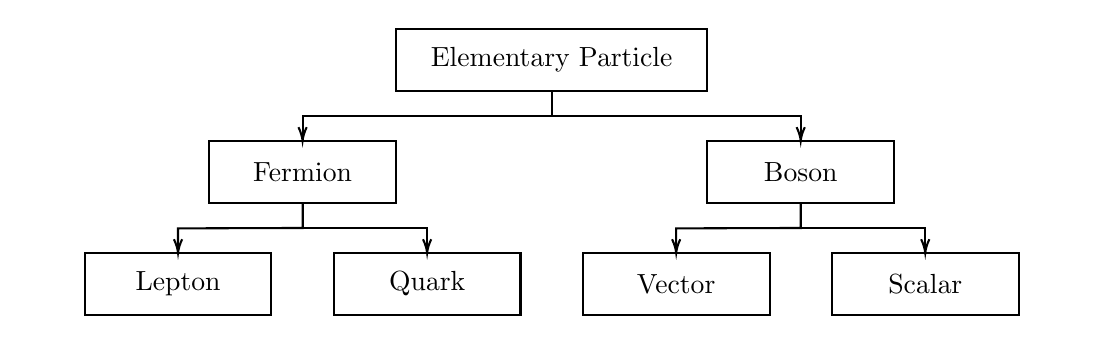
\begin{tikzpicture}[x=0.75pt,y=0.75pt,yscale=-0.6,xscale=0.6]
%uncomment if require: \path (0,306); %set diagram left start at 0, and has height of 306

%Flowchart: Process [id:dp696359542185788] 
\draw   (250,0) -- (500,0) -- (500,50) -- (250,50) -- cycle ;
%Flowchart: Process [id:dp8558192254273936] 
\draw   (100,90) -- (250,90) -- (250,140) -- (100,140) -- cycle ;
%Straight Lines [id:da09253439448016731] 
\draw    (375,50) -- (375,70) -- (175,70) -- (175,88) ;
\draw [shift={(175,90)}, rotate = 270] [color={rgb, 255:red, 0; green, 0; blue, 0 }  ][line width=0.75]    (10.93,-3.29) .. controls (6.95,-1.4) and (3.31,-0.3) .. (0,0) .. controls (3.31,0.3) and (6.95,1.4) .. (10.93,3.29)   ;
%Flowchart: Process [id:dp68005876657385] 
\draw   (500,90) -- (650,90) -- (650,140) -- (500,140) -- cycle ;
%Straight Lines [id:da33712707461320757] 
\draw    (375,50) -- (375,70) -- (575,70) -- (575,88) ;
\draw [shift={(575,90)}, rotate = 270] [color={rgb, 255:red, 0; green, 0; blue, 0 }  ][line width=0.75]    (10.93,-3.29) .. controls (6.95,-1.4) and (3.31,-0.3) .. (0,0) .. controls (3.31,0.3) and (6.95,1.4) .. (10.93,3.29)   ;
%Flowchart: Process [id:dp3110089650740445] 
\draw   (200,180) -- (350,180) -- (350,230) -- (200,230) -- cycle ;
%Flowchart: Process [id:dp3099562495446989] 
\draw   (0,180) -- (150,180) -- (150,230) -- (0,230) -- cycle ;
%Straight Lines [id:da28817746508352227] 
\draw    (175,140) -- (175,160) -- (75,160.33) -- (75,178) ;
\draw [shift={(75,180)}, rotate = 270] [color={rgb, 255:red, 0; green, 0; blue, 0 }  ][line width=0.75]    (10.93,-3.29) .. controls (6.95,-1.4) and (3.31,-0.3) .. (0,0) .. controls (3.31,0.3) and (6.95,1.4) .. (10.93,3.29)   ;
%Straight Lines [id:da0575641466520187] 
\draw    (175,140) -- (175,160) -- (275,160) -- (275,178) ;
\draw [shift={(275,180)}, rotate = 270] [color={rgb, 255:red, 0; green, 0; blue, 0 }  ][line width=0.75]    (10.93,-3.29) .. controls (6.95,-1.4) and (3.31,-0.3) .. (0,0) .. controls (3.31,0.3) and (6.95,1.4) .. (10.93,3.29)   ;
%Flowchart: Process [id:dp9199853601080596] 
\draw   (600,180) -- (750,180) -- (750,230) -- (600,230) -- cycle ;
%Flowchart: Process [id:dp3060126152626834] 
\draw   (400,180) -- (550,180) -- (550,230) -- (400,230) -- cycle ;
%Straight Lines [id:da9627421340802131] 
\draw    (575,140) -- (575,160) -- (475,160.33) -- (475,178) ;
\draw [shift={(475,180)}, rotate = 270] [color={rgb, 255:red, 0; green, 0; blue, 0 }  ][line width=0.75]    (10.93,-3.29) .. controls (6.95,-1.4) and (3.31,-0.3) .. (0,0) .. controls (3.31,0.3) and (6.95,1.4) .. (10.93,3.29)   ;
%Straight Lines [id:da7774551354270922] 
\draw    (575,140) -- (575,160) -- (675,160) -- (675,178) ;
\draw [shift={(675,180)}, rotate = 270] [color={rgb, 255:red, 0; green, 0; blue, 0 }  ][line width=0.75]    (10.93,-3.29) .. controls (6.95,-1.4) and (3.31,-0.3) .. (0,0) .. controls (3.31,0.3) and (6.95,1.4) .. (10.93,3.29)   ;

% Text Node
\draw (175,115) node   [align=left] {\begin{minipage}[lt]{102pt}\setlength\topsep{0pt}
\begin{center}
Fermion
\end{center}

\end{minipage}};
% Text Node
\draw (575,115) node   [align=left] {\begin{minipage}[lt]{102pt}\setlength\topsep{0pt}
\begin{center}
Boson
\end{center}

\end{minipage}};
% Text Node
\draw (275,205) node   [align=left] {\begin{minipage}[lt]{102pt}\setlength\topsep{0pt}
\begin{center}
Quark
\end{center}

\end{minipage}};
% Text Node
\draw (75,205) node   [align=left] {\begin{minipage}[lt]{102pt}\setlength\topsep{0pt}
\begin{center}
Lepton
\end{center}

\end{minipage}};
% Text Node
\draw (675,205) node   [align=left] {\begin{minipage}[lt]{102pt}\setlength\topsep{0pt}
\begin{center}
Scalar
\end{center}

\end{minipage}};
% Text Node
\draw (375,25) node   [align=left] {\begin{minipage}[lt]{102pt}\setlength\topsep{0pt}
\begin{center}
Elementary Particle
\end{center}

\end{minipage}};
% Text Node
\draw (475,205) node   [align=left] {\begin{minipage}[lt]{102pt}\setlength\topsep{0pt}
\begin{center}
Vector
\end{center}

\end{minipage}};
\end{tikzpicture}
\caption{Elementary particle classifications within the \gls{sm}.}
\label{fig:particle_classifications}
\end{figure}

Since neutrinos are neutral fermions, it is possible that neutrinos are their own antiparticle (a Majorana Particle). This idea was first proposed in 1937 by Majorana \cite{Majorana2020}. Within the \Gls{sm}, all fermions with the possible exception of neutrinos behave as Dirac fermions, that is, the particle and antiparticle are distinct \cite{dirac_majorana_neutrinos}. With the possibility that neutrinos are Majorana in nature, it has led to the search for neutrinoless double beta decay \cite{Double_beta_decay}. This is a variation on ordinary double beta decay in which a nucleus decays by emitting two electrons simultaneously. In ordinary double beta decay, there would also be two (anti)neutrinos in the final state, however, if neutrinos are Majorana particles, it can be thought of as one nucleon emitting a neutrino and the other absorbing it hence there are no neutrinos in the final state. Observation of such a decay would confirm the Majorana nature of neutrinos and give direct evidence for physics beyond the \Gls{sm} since the lepton number would not be conserved. Furthermore, neutrino oscillations (which is discussed in \SectionRef{subsec:Neutrino Oscillations}) are at odds with the \gls{sm} assumption that neutrinos are massless. With the requirement that neutrinos are indeed massive, the Dirac or Majorana nature of neutrinos is again discussed in \SectionRef{subsec:nutrino_mass} within the context of mass generation mechanisms \cite{The_physics_of_neutrinos_book}.

\subsection{Neutrinos within the Standard Model}

Neutrinos are a class of leptonic particle that only interact via the weak interaction and are considered massless within the \gls{sm}. It has been shown that \gls{cp} violation is allowed and exists within the \gls{sm}, however, the amount observed so far is insufficient to explain the matter-antimatter asymmetry. The amount of \gls{cp} violation associated with neutrinos, if any, is currently unknown, but may help explain the observed asymmetry. 

\subsubsection{Theory of Weak Interactions}\label{subsubsec:Theory of Weak Interactions}
The weak force is mediated by the charged W$^\pm$ and neutral Z$^0$ bosons. It is dubbed \textit{weak} because if the strong or \gls{em} forces are also present the weak force is usually subdominant. The active neutrinos only interact via the weak force (and gravity) which is one of the reasons they have been historically difficult to detect. 

One of the key components of the weak interaction relies on the concept of helicity of particles. The helicity of a particle is defined as the projection of its spin along the propagation direction.  If the spin is aligned with the direction of motion, the particle is said to be \textit{right-handed} and has an eigenvalue equal to +1 whereas if the spin is aligned in the opposite direction a particle is said to be \textit{left-handed} and has an eigenvalue equal to -1 \cite{MartinandShaw}. It was observed by Goldhaber and others that neutrinos appear to exclusively have left-handed helicities (and right-handed helicities for antineutrinos). The experiment they used to determine this was as follows; consider the decay of an isomer of europium via electron capture to an excited state of samarium. The samarium nucleus then decays to its ground state by emitting a photon. 
\begin{equation}
    ^{152m}Eu + e^- \longrightarrow {^{152}Sm^*} + \nue \longrightarrow ^{152}Sm + \gamma
\end{equation}
To conserve momentum, the excited samarium nucleus must recoil in a direction opposite to the emitted neutrino. To conserve angular momentum the spin of the neutrino and the recoiling nucleus must be in opposite directions which means that they both have the same handedness. Finally, the photon emitted will have a spin in the opposite direction to the neutrino and if the photon is emitted in a direction opposite to the neutrino direction, both will have the same helicity. The photons emitted in the direction opposite to the neutrino were identified, their helicity determined and it was found that they were all left-handed \cite{Goldhaber_experiment}. 

Helicity does commute with the Hamiltonian, however, it is not Lorentz invariant (for massive particles) \cite{Introduction_to_Particle_and_Astroparticle_Physics_book}. Since massive particles travel at speeds less than \textit{c}, it is always possible to boost to a frame such that the direction of motion is reversed. Spin is not affected by this which means that it is possible for the sign of the helicity to change. In contrast to helicity, chirality is a Lorentz invariant quantity that does not commute with the Hamiltonian. The chirality operator is $\gamma^5$ and it is defined as $i\gamma^0\gamma^1\gamma^2\gamma^3$ (i.e. \textit{i} times the product of the gamma matrices). Similarly to helicity, when the chirality operator acts on the eigenfunctions $\psi_R$ and $\psi_L$ it results in an eigenvalue of +1 and -1 respectively. It is commonly expressed in term of projection operators $P_{(L, R)}$ such that,
\begin{equation}
\begin{split}
    \psi_L &= P_L\psi \isdefined \frac{1-\gamma^5}{2}\psi \\
    \psi_R &= P_R\psi \isdefined \frac{1+\gamma^5}{2}\psi,
\end{split}
\end{equation}
where $\psi$ is a spinor which can be written in terms of left and right chiral components, $\psi = \psi_L + \psi_R$.
By defining $\overline{\psi} \equiv \psi^\dag \gamma^0$ and noting that $P_{(L,R)}^\hermitianT = P_{(L,R)}$ and $P_{(L,R)}\gamma^0 = \gamma^0P_{(R,L)}$, it follows that
\begin{equation}\label{eqn:chiral identity}
    \overline{\psi_L}\psi_L = \overline{\psi_R}\psi_R = 0.
\end{equation}
It should be noted that for massless particles, helicity is Lorentz invariant and becomes identical to chirality \cite{Fundamentals_of_Neutrino_Physics_and_Astrophysics}.

The weak force has two associated types of interaction: \gls{cc} interactions which are mediated by the charged W boson and \gls{nc} interactions which are mediated by the neutral Z boson. The defining difference is that for \gls{cc} interactions current flows between the interacting fermions (i.e. charge is exchanged), whereas for \gls{nc} interactions, the total flow of charge between the interacting fermions is zero. The weak component of the \gls{sm} Lagrangian is therefore comprised of two terms, one representing \gls{cc} and one representing \gls{nc}. The \gls{cc} current, $j^{CC}_{weak}$,  and \gls{nc} current, $j^{\gls{nc}}_{weak}$, components of each of these terms may be expressed as, 
\begin{equation}\label{eqn:weak current}
\begin{split}
    j^{CC}_{weak} &= \frac{g}{\sqrt{2}}\overline{\psi}\gamma^{\mu}P_L\psi, \\
    j^{NC}_{weak} &= \frac{g}{2\cos{\theta_W}}\sum_{i = \nu, l}
    \overline{\psi}_i \gamma^\mu (g_V^i - g_A^i \gamma^5)\psi_i, 
\end{split}
\end{equation}
where $g$ is the weak coupling factor, $\theta_W$ is the Weinberg angle, $g_V$ is the vector coupling and $g_A$ is the axial coupling \cite{Particles_and_Fundamental_Interactions:_An_Introduction_to_Particle_Physics}\cite{Fundamentals_of_Neutrino_Physics_and_Astrophysics}\cite{PDG_2022}. The weak coupling is related to the Fermi Constant, $G_F$, and the boson masses such that,
\begin{equation}
\begin{split}
    \frac{g^2}{8m^2_W} &= \frac{G_F}{\sqrt{2}}, \\
    \frac{g^2}{8m^2_Z\cos^2{\theta_W}} &= \frac{G_F}{\sqrt{2}},
\end{split}
\end{equation}
where $m_W$ is the mass of the W boson and $m_Z$ is the mass of the Z boson \cite{Fundamentals_of_Neutrino_Physics_and_Astrophysics}.

$j^{CC}_{weak}$ has the form of a vector-axial (V--A) interaction, where the vector current is given by $\overline{\psi}\gamma^\mu\psi$ and the axial current is given by $\overline{\psi}\gamma^\mu\gamma^5\psi$. The axial component remains unchanged under a parity transformation, whereas the sign of the vector component changes. Usually, the square of the amplitude is of interest, which in short means taking the square of the weak current. This results in a squared vector and axial component plus a cross-term. Since the axial and vector components behave differently under a parity transformation, this cross term leads to parity violation \cite{Particles_and_Fundamental_Interactions:_An_Introduction_to_Particle_Physics} \cite{Fundamentals_of_Neutrino_Physics_and_Astrophysics}. $j^{NC}_{weak}$ does not have the form of a V--A interaction, but does again have both vector and axial components which lead to parity violation \cite{Particles_and_Fundamental_Interactions:_An_Introduction_to_Particle_Physics}.

\begin{comment}
Because the projection operator, $P_L$, appears in \EquationRef{eqn:weak current} it follows that weak interactions only apply to left-handed particles (and right-handed antiparticles).
\end{comment}

The \gls{sm} is constructed such that only the left components of the field couple to the W and Z bosons so it follows that only left-handed particles (and right-handed antiparticles) can weakly interact. Neutrinos only interact via the weak force which means they are therefore produced with a left-handed chirality and since they are ultra-relativistic, for all intents and purposes they also have a left-handed helicity. Additionally, a neutrino that is present in a weak interaction is always in a definite flavour state which corresponds to the associated charged lepton (therefore conserving lepton number) \cite{Quarks_and_Leptons:_An_Introductor_Course_in_Modern_Particle_Physics_book}.

\subsubsection{Weak Interaction Processes}

The following section outlines some of the most common \gls{cc} and \gls{nc} interaction processes. The associated \gls{cc} and \gls{nc} Feynman diagrams for these processes are shown in \FigureRef{fig:CC_Feynman_diagrams} and \FigureRef{fig:NC_Feynman_diagrams} respectively (the possible \gls{2p2h} interactions are shown separately in \FigureRef{fig:mec_feynman_diagrams}). Only examples of neutrino interactions are shown, however, these may be easily adapted to the antineutrino case. Additionally, interaction flavours are kept general with \textit{l} representing the lepton flavour.

\paragraph{Elastic and Quasi-Elastic}
When particles interact via elastic scattering, the initial particles do not change. Since neutrinos are neutral particles that weakly interact, \gls{nc} elastic scattering being mediated by the Z$^0$ boson may occur with a neutrino scattering off a proton via
\begin{equation}
    \nu_l + p \rightarrow \nu_l + p.
\end{equation}

Quasi-elastic scattering is similar to elastic scattering, however, charge is exchanged and therefore the interaction is mediated by the W$^+$ boson. \gls{ccqe} interactions are defined by the production of a charged lepton plus a (semi-) stable baryon. The dominant form of these interactions occur when the incoming neutrino scatters off a neutron and is converted to its charged lepton counterpart whilst the neutron changes to a proton via
\begin{equation}
    \nu_l + n \rightarrow l^- + p.
\end{equation}
\gls{ccqe} interactions are the most abundant in the GeV range, which is the energy range of the \gls{bnb} \cite{Measurement_of_the_Antineutrino_Double-Differential_Charged-Current_Quasi-Elastic_Scattering_Cross_Section_at_MINERvA_book}. 

\paragraph{Resonant}
At higher energies, the neutrino-nucleon interaction may cause the nucleon to be excited into a baryon resonance. The resonance will then decay back into a nucleon plus a pion. Using the Delta resonance (Delta baryon) as an example, \gls{cc} interaction occur via
\begin{equation}
    \nu_l + N \rightarrow l^- + \Delta \rightarrow l^- + N + \pi,
\end{equation}
whereas \gls{nc} interactions occur via,
\begin{equation}
    \nu_l + N \rightarrow \nu_l + \Delta \rightarrow \nu_l + N +\pi.
\end{equation}
In both cases, \textit{N} represents some nucleon with $\Delta$ and $\pi$ being one of the possible Delta resonances and pions appropriate for a given interaction \cite{Measurement_of_the_Antineutrino_Double-Differential_Charged-Current_Quasi-Elastic_Scattering_Cross_Section_at_MINERvA_book} \cite{Measurement_of_the_Water_to_Scintillator_Charged-Current_Cross-Section_Ratio_for_Muon_Neutrinos_at_the_T2K_Near_Detector_thesis}. 

\paragraph{2 Particles 2 Holes}
Within the nuclear environment, there is a correlation between the distribution of nucleons. Therefore, some of the nucleons are bounded in pairs and these bound nucleon pairs may be thought of as being bound due to the exchange of virtual mesons.\footnote{This exchange of mesons is sometimes also known as a \gls{mec}. \glspl{mec} are a subset of \gls{2p2h} interaction where the W boson couples directly to the exchanged meson, however, these terms are sometimes used interchangeably.} In this type of interaction, multiple nucleons are excited in a quasi-elastic fashion. The boson may couple to either a nucleon or the meson that is being exchanged. This leads to a number of possibilities such as; 1) the boson couples to the exchanged meson (pion-in-flight diagram), 2) the boson couples at the vertex between the nucleon and exchanged meson (seagull diagram), 3) the meson exchange occurs with a virtual intermediate nucleon to which the boson couples, 4) as in case 3), but the intermediate particle is a Delta resonance instead of a nucleon. Feynman diagrams of these 4 possibilities are shown in \FigureRef{fig:mec_feynman_diagrams} \cite{Measurement_of_the_Antineutrino_Double-Differential_Charged-Current_Quasi-Elastic_Scattering_Cross_Section_at_MINERvA_book}\cite{Adjusting_neutrino_interaction_models_and_evaluating_uncertainties_using_NOvA_near_detector_data}
\cite{Seagull_and_pion-in-flight_mec}.

\begin{figure}
\begin{subfigure}{0.4\linewidth}
\resizebox{0.8\linewidth}{4cm}{
\begin{feynman}
    \weak[color=FFFFFF]{13.50, 4.00}{15.00, 5.50} % Draw invisible line so it has the same "shape" as the other diagrams
    \dashed[label=$\pi$, labelDistance=0.3, showArrow=false]{15.00, 6.50}{17.00, 6.50}
    \fermion[label=$N_2$, labelDistance=0.1, labelLocation=0.1, showArrow=true]{17.00, 4.00}{17.00, 6.00}
    \fermion[showArrow=true]{15.00, 6.00}{15.00, 8.00}
    \fermion[label=$N_1$, labelDistance=0.1, labelLocation=0.1, showArrow=true]{15.00, 4.00}{15.00, 6.00}
    \fermion[showArrow=true]{17.00, 6.00}{17.00, 8.00}
    \weak[label=$W$, labelDistance=0.3]{16.00, 4.00}{16.00, 6.5}
\end{feynman}
}
\caption{}
\end{subfigure}
\begin{subfigure}{0.4\linewidth}
\resizebox{0.8\linewidth}{4cm}{
\begin{feynman}
    \dashed[label=$\pi$, labelDistance=0.3, showArrow=false]{15.00, 6.00}{17.00, 6.00}
    \fermion[label=$N_2$, labelDistance=0.1, labelLocation=0.1, showArrow=true]{17.00, 4.00}{17.00, 6.00}
    \fermion[showArrow=true]{15.00, 6.00}{15.00, 8.00}
    \fermion[label=$N_1$, labelDistance=0.1, labelLocation=0.1, showArrow=true]{15.00, 4.00}{15.00, 6.00}
    \fermion[showArrow=true]{17.00, 6.00}{17.00, 8.00}
    \weak[label=$W$, labelDistance=0.6]{13.50, 4.50}{15.00, 6.00}
\end{feynman}
}
\caption{}
\end{subfigure}
\vspace{0.5cm}
\begin{subfigure}{0.4\linewidth}
\resizebox{0.8\linewidth}{4cm}{
\begin{feynman}
    \dashed[label=$\pi$, labelDistance=0.3, showArrow=false]{15.00, 6.50}{17.00, 6.50}
    \fermion[label=$N_2$, labelDistance=0.1, labelLocation=0.1, showArrow=true]{17.00, 4.00}{17.00, 6.00}
    \fermion[showArrow=true]{15.00, 6.00}{15.00, 8.00}
    \fermion[label=$N_1$, labelDistance=0.1, labelLocation=0.1, showArrow=true]{15.00, 4.00}{15.00, 6.00}
    \fermion[showArrow=true]{17.00, 6.00}{17.00, 8.00}
    \weak[label=$W$, labelDistance=0.6]{13.50, 4.00}{15.00, 5.50}
\end{feynman}
}
\caption{}
\end{subfigure}
\begin{subfigure}{0.4\linewidth}
\resizebox{0.8\linewidth}{4cm}{
\begin{feynman}
    \dashed[label=$\pi$, labelDistance=0.3, showArrow=false]{15.00, 6.50}{17.00, 6.50}
    \fermion[label=$N_2$, labelDistance=0.1, labelLocation=0.1, showArrow=true]{17.00, 4.00}{17.00, 6.00}
    \fermion[showArrow=true]{15.00, 6.00}{15.00, 8.00}
    \fermion[label=$\Delta$, labelDistance=-0.5, showArrow=false, lineWidth=6]{15.00, 5.50}{15.00, 6.50}
    \fermion[label=$N_1$, labelDistance=0.1, labelLocation=0.1, showArrow=true]{15.00, 4.00}{15.00, 6.00}
    \fermion[showArrow=true]{17.00, 6.00}{17.00, 8.00}
    \weak[label=$W$, labelDistance=0.6]{13.50, 4.00}{15.00, 5.50}
\end{feynman}
}
\caption{}
\end{subfigure}
 \caption[Feynman diagrams of possible \gls{2p2h} interactions.]{Feynman diagrams of possible \gls{2p2h} interactions. The boson may couple to (a) the pion-in-flight, (b) the \gls{2p2h} vertex (seagull diagram), (c) an intermediate nucleon, (d) an intermediate Delta resonance \cite{Measurement_of_the_Antineutrino_Double-Differential_Charged-Current_Quasi-Elastic_Scattering_Cross_Section_at_MINERvA_book}.}
\label{fig:mec_feynman_diagrams}
\end{figure}

\begin{comment}
\begin{figure}[h!]
    \centering
    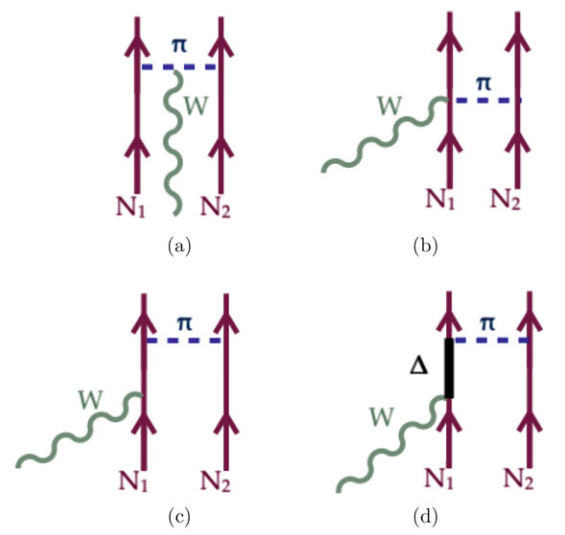
\includegraphics[width = \largefigwidth]{figures-chap3/mec_diagrams.png}
    \caption[Feynman diagrams of possible \gls{mec} interactions.]{Feynman diagrams of possible \gls{mec} interactions. The boson may couple to (a) the pion-in-flight, (b) the \gls{mec} vertex (seagull diagram), (c) an intermediate nucleon, (d) an intermediate Delta resonance \cite{Measurement_of_the_Antineutrino_Double-Differential_Charged-Current_Quasi-Elastic_Scattering_Cross_Section_at_MINERvA_book}.}
    \label{fig:mec_feynman_diagrams}
\end{figure}
\end{comment}

\newpage
\paragraph{Deep Inelastic Scattering}
At even higher energies than those for resonant interactions ($>\mathcal{O}$(5 GeV)), \gls{dis} interactions become dominant. In \gls{dis} interactions, the neutrino scatters off individual quarks rather than the nucleon as a whole. This results in the breakup of the nucleon, but since the strong force prevents single quarks from existing, a hadronic shower \textit{X} is produced \cite{Fundamentals_of_Neutrino_Physics_and_Astrophysics} \cite{Measurement_of_the_Antineutrino_Double-Differential_Charged-Current_Quasi-Elastic_Scattering_Cross_Section_at_MINERvA_book}. A \gls{cc} \gls{dis} interaction occurs via
\begin{equation}
    \nu_l + N \rightarrow l^- + X,
\end{equation}
whereas the \gls{nc} interaction occurs via
\begin{equation}
    \nu_l + N \rightarrow \nu_l + X.
\end{equation}


\paragraph{Coherent Production}
Coherent interactions occur when the neutrino scatters off the whole nucleus with a negligible momentum transfer. This results in final state particles such as pions, rho mesons or photons being produced, but leaves the target nucleus unaltered. Coherent scattering may occur for both \gls{cc} and \gls{nc} interactions (with pions in the final state being used as an example) via
\begin{equation}
    \nu_l + A \rightarrow l^- + A + \pi^+
\end{equation}
and
\begin{equation}
    \nu_l + A \rightarrow \nu_l + A + \pi^0
\end{equation}
respectively \cite{Measurement_of_the_Water_to_Scintillator_Charged-Current_Cross-Section_Ratio_for_Muon_Neutrinos_at_the_T2K_Near_Detector_thesis}\cite{Adjusting_neutrino_interaction_models_and_evaluating_uncertainties_using_NOvA_near_detector_data}. 


\paragraph{Neutrino Electron Scattering}
Instead of scattering off the nucleus, neutrinos may also scatter off the electrons in an atom via,
\begin{equation}
    \nu_l + \electron \rightarrow \nu_l + \electron.
\end{equation}
This is an elastic process that has indistinguishable \gls{cc} and \gls{nc} components for \nue interactions, whereas only a \gls{nc} component is allowed for \numu and \nutau \cite{Fundamentals_of_Neutrino_Physics_and_Astrophysics}.

%https://feynman.aivazis.com/
\newpage
\begin{figure}[h!]
\centering
\begin{subfigure}{0.3\linewidth}
\vspace{0.3cm}
\centering \textbf{CC QE} \\ \vspace{0.3cm}
\resizebox{\linewidth}{4cm}{
\begin{feynman}
    \fermion[label=$l$, labelDistance=0.3, showArrow=true, flip=false]{6.00, 8.00}{8.00, 9.00}
    \fermion[label=$\nu_l$, labelDistance=0.2]{4.00, 9.00}{6.00, 8.00}
    \weak[color=000000, label=$W^+$, labelDistance=0.3]{6.00, 8.00}{6.00, 6.00}
    \fermion[label=$p$, labelDistance=0.2, showArrow=true]{6.00, 6.00}{8.00, 5.00}
    \fermion[label=$n$, labelDistance=0.3, showArrow=true]{4.00, 5.00}{6.00, 6.00}
\end{feynman}
}
\end{subfigure} 
\begin{subfigure}{0.3\linewidth}
\vspace{0.3cm}
\centering \textbf{CC Res} \\ \vspace{0.3cm}
\resizebox{\linewidth}{4cm}{
\begin{feynman}
    \fermion[label=$l$, labelDistance=0.3, showArrow=true, flip=false]{6.00, 8.00}{8.00, 9.00}
    \fermion[label=$\nu_l$, labelDistance=0.2]{4.00, 9.00}{6.00, 8.00}
    \weak[color=000000, label=$W^+$, labelDistance=0.3]{6.00, 8.00}{6.00, 6.00}
    \fermion[label=$N$, labelDistance=0.3, showArrow=true, flip=true]{6.00, 6.00}{4.00, 5.00}
    \dashed[label=$\Delta$, labelDistance=0.2]{6.00, 6.00}{7.00, 5.50}
    \fermion[label=$N$, labelDistance=0.2]{7.00, 5.50}{8.00, 5.00}
    \fermion[label=$\pi$,labelDistance=0.3]{7.00, 5.50}{8.00, 6.00}
\end{feynman}
}
\end{subfigure}\\
\begin{comment}
\vspace{1cm}
\begin{subfigure}{0.3\linewidth}
\centering \textbf{CC MEC} \\ \vspace{0.3cm}
\resizebox{\linewidth}{4cm}{
\begin{feynman}
    \fermion[label=$l$, labelDistance=0.3, showArrow=true, flip=false]{6.00, 8.00}{8.00, 9.00}
    \fermion[label=$\nu_l$, labelDistance=0.2]{4.00, 9.00}{6.00, 8.00}
    \weak[color=000000, label=$W^+$, labelDistance=0.3]{6.00, 8.00}{6.00, 6.00}
    \fermion[label=$n$, labelDistance=0.4, showArrow=true, flip=true]{6.00, 6.00}{4.00, 5.00}
    \fermion[label=$p$, labelDistance=0.3]{6.00, 6.00}{8.00, 5.00}
    \fermion[label=$p$, labelDistance=0.4]{4.00, 4.00}{6.00, 5.00}
    \dashed[showArrow=false, label=$\pi^+$, labelDistance=0.1]{6.00, 5.00}{6.00, 6.00}
    \fermion[label=$p$, labelDistance=0.3]{6.00, 5.00}{8.00, 4.00}
\end{feynman}
}
\end{subfigure}
\end{comment}
\begin{subfigure}{0.3\linewidth}
\vspace{0.3cm}
\centering \hspace{0cm} \textbf{CC DIS} \\ \vspace{0.3cm}
\resizebox{1.1\linewidth}{4cm}{
\begin{feynman}
    \fermion[label=$l$, labelDistance=0.3, showArrow=true, flip=false]{24.00, 12.00}{26.00, 13.00}
    \fermion[label=$\nu_l$, labelDistance=0.2]{22.00, 13.00}{24.00, 12.00}
    \fermion[label=$N$, labelDistance=0.4]{22.00, 9.00}{23.70, 10.00}
    \weak[color=000000, label=$W^+$, labelDistance=0.3]{24.00, 10.30}{24.00, 12.00}
    \fermion[]{24.30, 10.00}{26.00, 10.5}
    \fermion[]{24.30, 10.00}{26.00, 10.00}
    \fermion[]{24.30, 10.00}{26.00, 9.5}
    \parton{24.00,10.00}{0.30}
    \textfeynman{26.3,10}{\textbf{X}}
\end{feynman}
}
\end{subfigure}
%\hspace{-0.6cm}
\begin{subfigure}{0.3\linewidth}
\vspace{0.3cm}
\centering \textbf{CC Coh} \\ \vspace{0.3cm}
\resizebox{\linewidth}{4cm}{
\begin{feynman}
    \fermion[label=$l$, labelDistance=0.3, showArrow=true, flip=false]{24.00, 12.00}{26.00, 13.00}
    \fermion[label=$\nu_l$, labelDistance=0.2]{22.00, 13.00}{24.00, 12.00}
    \fermion[label=$A$, labelDistance=0.4]{22.00, 9.00}{23.70, 10.00}
    \weak[color=000000, label=$W^+$, labelDistance=0.3]{24.00, 11.15}{24.00, 12.00}
    \dashed[showArrow=false, color=000000, labelDistance=0.3]{24.00, 10.3}{24.00, 11.15}
    \fermion[label=$\pi^+$, labelDistance=0.3]{24.00, 11.15}{26.00, 11.15}
    \fermion[label=$A$, labelDistance=0.2]{24.30, 10.00}{26.00, 10.0}
    \parton{24.00,10.00}{0.30}
\end{feynman}
}
\end{subfigure}
\begin{subfigure}{0.3\linewidth}
\vspace{0.3cm}
\centering \textbf{CC \electron Scat} \\ \vspace{0.3cm}
\resizebox{\linewidth}{4cm}{
\begin{feynman}
    \fermion[label=$\electron$, labelDistance=0.3, showArrow=true, flip=false]{24.00, 12.00}{26.00, 13.00}
    \fermion[label=$\nue$, labelDistance=0.2]{22.00, 13.00}{24.00, 12.00}
    \weak[color=000000, label=$W^+$, labelDistance=0.3]{24.00, 10.00}{24.00, 12.00}
    \fermion[label=$\nue$, labelDistance=0.2, showArrow=true]{24.00, 10.00}{26.00, 9.00}
    \fermion[label=$\electron$, labelDistance=0.3, showArrow=true]{22.00, 9.00}{24.00, 10.00}
\end{feynman}
}
\end{subfigure}
\caption[Feynman diagrams of the \gls{cc} processes most commonly expected in \gls{sbn}.]{Feynman diagrams of the \gls{cc} processes most commonly expected in \gls{sbn}. $\nu_l$ corresponds to the neutrino with leptonic flavour \textit{l}, with \textit{l} typically being either an electron or a muon. $\Delta$ denotes one of the possible Delta resonances, \textit{N} denotes a nucleon, \textit{X} denotes some set of final hadrons and \textit{A} denotes a nucleus.}
\label{fig:CC_Feynman_diagrams}
\end{figure}

\newpage
\begin{figure}[h!]
\begin{subfigure}{0.3\linewidth}
\centering \textbf{NC Elastic} \\ \vspace{0.3cm}
\resizebox{\linewidth}{4cm}{
\begin{feynman}
    \fermion[label=$\nu_l$, labelDistance=0.3]{6.00, 7.00}{8.00, 8.00}
    \fermion[label=$\nu_l$, labelDistance=0.2]{4.00, 8.00}{6.00, 7.00}
    \weak[color=000000, label=$Z^0$, labelDistance=0.3]{6.00, 7.00}{6.00, 5.00}
    \fermion[label=$p$, labelDistance=0.3]{4.00, 4.00}{6.00, 5.00}
    \fermion[label=$p$, labelDistance=0.2]{6.00, 5.00}{8.00, 4.00}
\end{feynman}
}
\end{subfigure}
\begin{subfigure}{0.3\linewidth}
\centering \textbf{NC Res} \\ \vspace{0.3cm}
\resizebox{\linewidth}{4cm}{
\begin{feynman}
    \fermion[label=$\nu_l$, labelDistance=0.3, showArrow=true, flip=false]{6.00, 8.00}{8.00, 9.00}
    \fermion[label=$\nu_l$, labelDistance=0.2]{4.00, 9.00}{6.00, 8.00}
    \weak[color=000000, label=$Z^0$, labelDistance=0.3]{6.00, 8.00}{6.00, 6.00}
    \fermion[label=$N$, labelDistance=0.3, showArrow=true, flip=true]{6.00, 6.00}{4.00, 5.00}
    \dashed[label=$\Delta$, labelDistance=0.2]{6.00, 6.00}{7.00, 5.50}
    \fermion[label=$N$, labelDistance=0.2]{7.00, 5.50}{8.00, 5.00}
    \fermion[label=$\pi$,labelDistance=0.3]{7.00, 5.50}{8.00, 6.00}
\end{feynman}
}
\end{subfigure}\\
\begin{comment}
\vspace{1cm}
\begin{subfigure}{0.3\linewidth}
\centering \textbf{NC MEC} \\ \vspace{0.3cm}
\resizebox{\linewidth}{4cm}{
\begin{feynman}
    \fermion[label=$\nu_l$, labelDistance=0.3, showArrow=true, flip=false]{6.00, 8.00}{8.00, 9.00}
    \fermion[label=$\nu_l$, labelDistance=0.2]{4.00, 9.00}{6.00, 8.00}
    \weak[color=000000, label=$Z^0$, labelDistance=0.3]{6.00, 8.00}{6.00, 6.00}
    \fermion[label=$n$, labelDistance=0.4, showArrow=true, flip=true]{6.00, 6.00}{4.00, 5.00}
    \fermion[label=$n$, labelDistance=0.3]{6.00, 6.00}{8.00, 5.00}
    \fermion[label=$p$, labelDistance=0.4]{4.00, 4.00}{6.00, 5.00}
    \dashed[showArrow=false, label=$\pi^0$, labelDistance=0.1]{6.00, 5.00}{6.00, 6.00}
    \fermion[label=$p$, labelDistance=0.3]{6.00, 5.00}{8.00, 4.00}
\end{feynman}
}
\end{subfigure}
\end{comment}
\begin{subfigure}{0.3\linewidth}
\vspace{0.3cm}
\centering \hspace{-0cm}\textbf{NC DIS} \\ \vspace{0.3cm}
\resizebox{1.1\linewidth}{4cm}{
\begin{feynman}
    \fermion[label=$\nu_l$, labelDistance=0.3, showArrow=true, flip=false]{24.00, 12.00}{26.00, 13.00}
    \fermion[label=$\nu_l$, labelDistance=0.2]{22.00, 13.00}{24.00, 12.00}
    \fermion[label=$N$, labelDistance=0.4]{22.00, 9.00}{23.70, 10.00}
    \weak[color=000000, label=$Z^0$, labelDistance=0.3]{24.00, 10.30}{24.00, 12.00}
    \fermion[]{24.30, 10.00}{26.00, 10.50}
    \fermion[]{24.30, 10.00}{26.00, 10.00}
    \fermion[]{24.30, 10.00}{26.00, 9.50}
    \parton{24.00,10.00}{0.30}
    \textfeynman{26.3,10}{\textbf{X}}
\end{feynman}
}
\end{subfigure}
%\hspace{-0.6cm}
\begin{subfigure}{0.3\linewidth}
\vspace{0.3cm}
\centering \textbf{NC Coh} \\ \vspace{0.3cm}
\resizebox{\linewidth}{4cm}{
\begin{feynman}
    \fermion[label=$\nu_l$, labelDistance=0.3, showArrow=true, flip=false]{24.00, 12.00}{26.00, 13.00}
    \fermion[label=$\nu_l$, labelDistance=0.2]{22.00, 13.00}{24.00, 12.00}
    \fermion[label=$A$, labelDistance=0.4]{22.00, 9.00}{23.70, 10.00}
    \weak[color=000000, label=$Z^0$, labelDistance=0.3]{24.00, 11.15}{24.00, 12.00}
    \dashed[showArrow=false, color=000000, labelDistance=0.3]{24.00, 10.30}{24.00, 11.15}
    \fermion[label=$\pi^0$, labelDistance=0.3]{24, 11.15}{26.00, 11.15}
    \fermion[label=$A$, labelDistance=0.2]{24.30, 10.00}{26.00, 10.00}
    \parton{24.00,10.00}{0.30}
\end{feynman}
}
\end{subfigure}
\begin{subfigure}{0.3\linewidth}
\vspace{0.3cm}
\centering \textbf{NC \electron Scat} \\ \vspace{0.3cm}
\resizebox{\linewidth}{4cm}{
\begin{feynman}
    \fermion[label=$\nu_l$, labelDistance=0.3, showArrow=true, flip=false]{24.00, 12.00}{26.00, 13.00}
    \fermion[label=$\nu_l$, labelDistance=0.2]{22.00, 13.00}{24.00, 12.00}
    \weak[color=000000, label=$Z^0$, labelDistance=0.3]{24.00, 10.00}{24.00, 12.00}
    \fermion[label=$\electron$, labelDistance=0.2, showArrow=true]{24.00, 10.00}{26.00, 9.00}
    \fermion[label=$\electron$, labelDistance=0.3, showArrow=true]{22.00, 9.00}{24.00, 10.00}
\end{feynman}
}
\end{subfigure}
\caption[Feynman diagrams of the \gls{nc} processes most commonly expected in \gls{sbn}.]{Feynman diagrams of the \gls{nc} processes most commonly expected in \gls{sbn}. $\nu_l$ corresponds to the neutrino with leptonic flavour \textit{l}, with \textit{l} typically being either an electron or a muon. $\Delta$ denotes one of the possible Delta resonances, \textit{N} denotes a nucleon, \textit{X} denotes some set of final hadrons and \textit{A} denotes a nucleus.}
\label{fig:NC_Feynman_diagrams}
\end{figure}

\subsubsection{CP Violation}\label{subsubsec:CP_violation}

It was shown experimentally by Wu that \gls{p} conservation is violated and later by Cronin and Fitch that \gls{cp} conservation is also violated \cite{Wu_experiment}\cite{Cronin_and_Fitch_experiment}. \gls{cp} violation is one of the Sakharov conditions required to have a matter-antimatter asymmetry in the universe, however, the amount of \gls{cp} violation that has currently been observed is seemingly insufficient to explain the matter-dominated universe that is observed \cite{Sakharov_conditions}.

Currently, essentially all the \gls{cp} violation that has been experimentally confirmed arises from the \gls{ckm} in the quark sector. The \gls{ckm} is a unitary matrix that gives a measure of the strength of flavour changes for quarks in weak interactions. Before the discovery of the third generation of quarks, the "\gls{ckm}", was simply a $2 \times 2$ rotation matrix known as the Cabibbo matrix defined in terms of the Cabibbo angle. For a $N \times N$ unitary matrix, there are $(N-1)^2$ free parameters. $\frac{1}{2}N(N-1)$ parameters are rotation angles (mixing angles) and the remaining $\frac{1}{2}(N-1)(N-2)$ parameters (assuming Dirac particles) are complex phases resulting in \gls{cp} violation. For the case of the Cabibbo matrix there is only one mixing angle, which is the Cabibbo angle and no complex phase \cite{Fundamentals_of_Neutrino_Physics_and_Astrophysics} \cite{leptonic_cp_violation}. 

\gls{cp} violation had been observed in Kaon decays as early as 1964, which was before the discovery of the bottom quark \cite{Cronin_and_Fitch_experiment}. Kobayashi and Maskawa proposed the existence of a third-generation of quarks in order to explain \gls{cp} violation since a $3\times3$ matrix is required to generate a \gls{cp} violating term \cite{CP_Violation_in_the_Renormalizable_Theory_of_Weak_Interaction}. The bottom quark was then experimentally discovered in 1977 later followed by the top quark to complete the quark pairs of each generation \cite{bottom_quark_discovery}. 

The strong interaction appears not to violate \gls{cp}, despite seemingly having the possibility to do so. As there is currently no explanation for why the strong force does not violate \gls{cp}, it has been dubbed the \textit{Strong \gls{cp} Problem} and is an example of fine-tuning. An experimental example of the strong force conserving \gls{cp} is the case of no electric dipole moment being observed in neutrons. The electric dipole moment predicted by the strong interaction if \gls{cp} were to be violated far exceeds the upper bound that has been experimentally found \cite{strong_CP_problem}.

Since the strong interaction appears to conserve \gls{cp} and the \gls{cp} violation in the quark sector is insufficient to explain the matter-antimatter asymmetry observed, an additional source is required. Similar to how the \gls{ckm} matrix gives a measure of flavour changes in quarks, the \gls{pmns} matrix gives a measure of mixing in neutrinos and may provide a source of \gls{cp} violation in the lepton sector. The confirmation of the 3 generations of neutrinos again gives rise to a complex \gls{cp} violating Dirac phase. The amount of \gls{cp} violation in the neutrino sector is largely unconstrained with the current best fit value for $\delta_{CP}/^\circ$ being $197^{+0.21}_{-0.2}$ for the normal hierarchy and $286^{+27}_{-32}$ for the inverted hierarchy \cite{nu_ft_v2}. One of the primary aims of future long baseline neutrino experiments such as Hyper-Kamiokande and \gls{dune} will be to measure \gls{cp} violation from the Dirac phase \cite{Hyper_Kamiokande_design_report}\cite{DUNE_design_report}. If the Majorana nature of neutrinos is confirmed, additional sources of \gls{cp} violation may be present. Unlike Dirac particles, the number of phases associated with Majorana particles is given by $\frac{1}{2}N(N-1)$, meaning for a three neutrino model, there are two additional \gls{cp} violating terms \cite{Majorana_neutrinos_and_other_Majorana_particles_Theory_and_experiment}.


 

\subsection{Neutrino Masses}\label{subsec:nutrino_mass}

Assuming that the mass generation of neutrinos follows similar rules to that of other Dirac mass terms, there is motivation to try and attempt to include sterile neutrinos into theoretical models since right-handed fields are required. Some of the potential options for neutrino mass generation are discussed below. The initial mass scale for sterile neutrinos is unconstrained, however, one of the more well-motivated models is the "Type 1" \textit{seesaw model} which attempts to explain the relative size of neutrino masses and points towards very heavy sterile neutrino masses ($\gg ~1$ eV). Variations of the Seesaw model have also been proposed that incorporate light sterile neutrinos \cite{White_Paper}.

The \gls{sm} Lagrangian, $\mathcal{L}$, for a fermion is given by
\begin{equation}\label{eqn:SM Lagrangian}
    \mathcal{L} = \overline{\psi}(i\gamma^{\mu} \partial_{\mu} - m)\psi
\end{equation}
with the associated Euler-Lagrange equation being the Dirac equation which is given by \cite{Fundamentals_of_Neutrino_Physics_and_Astrophysics}
\begin{equation}
    (i\gamma^\mu\partial_\mu - m)\psi = 0.
\end{equation}
\subsubsection{Dirac Mass}
Within the \gls{sm} Lagrangian, the Dirac mass term is given by $m_D\overline{\psi}\psi$ where $\psi$ is the Dirac spinor. By dividing this into left and right components it follows that
\begin{equation}\label{eqn:Dirac mass term}
\begin{split}
    m_D\overline{\psi}\psi &= m_D(\overline{\psi_L + \psi_R})(\psi_L + \psi_R) \\
    &= m_D(\overline{\psi_L}\psi_R + \overline{\psi_R}\psi_L),
\end{split}
\end{equation} 
where the second step follows from \EquationRef{eqn:chiral identity}. Naturally, to have a non-zero Dirac mass term, particles require a left and right-handed chiral state. This is the mass generation method that all particles in the \gls{sm} follow and hence why neutrinos are massless in the \gls{sm}. To give the neutrino mass in this way, a field associated with a right-handed neutrino could be introduced. This would usually correspond to the left-handed neutrinos being the \textit{active} ones, whilst the right-handed neutrinos would be considered \textit{sterile}.
\begin{comment}
Since left handed particles form a doublet under \SUgroup2 they have non-zero weak isospin and because right handed particles are a singlet under \SUgroup2, their weak isospin is equal to zero. Therefore, in order to get a term where the isospin sums to zero, which is a requirement for the Lagrangian to be gauge invariant, an additional field is needed that is also a doublet under \SUgroup2. This field is a result of the neutral Higgs boson, $\phi^0$, and the Dirac mass is given by
\end{comment}
Yukawa coupling can be introduced between the lepton doublets and the Higgs doublet include right handed neutrinos. After spontaneous symmetry breaking, this gives rise to a Dirac mass term whch is given by, \begin{equation}
    {m_D}_i = \frac{y_iv}{\sqrt{2}},
\end{equation}
where \textit{y} is the Yukawa coupling and \textit{v} gives the vacuum expectation value from the Higgs field ($v \simeq$ 246 GeV) \cite{peskin_and_schroeder}. A concern with generating neutrino masses in this way is the required size of the Yukawa coupling. To generate a mass of say 0.1 eV, the Yukawa coupling would need to be very small ($\sim$6 orders of magnitude less than that of the electron). This small number is sometimes considered unnatural and provides motivation to search for alternative mass mechanisms to explain the neutrino masses \cite{Fundamentals_of_Neutrino_Physics_and_Astrophysics}.

\subsubsection{Majorana Mass}
To generate mass without the requirement of a right-handed field, it is required that the neutrino be a Majorana particle. It may be shown that 
\begin{equation}
    P_R C\overline{\psi_L}^T = C\overline{\psi_L}^T,
\end{equation}
which means that $C\overline{\psi_L}^T$ is a right handed object, where the superscript \textit{T} indicates the transpose and $C = i \gamma^2 \gamma^0$ which is the charge conjugation operator. By defining $\psi_L^C = C\overline{\psi_L}^T$, the Majorana field mass term in the Lagrangian can be written as
\begin{equation}\label{eqn:Majorana mass term}
    \frac{m_L}{2}(\overline{\psi_L^C}\psi_L + \overline{\psi_L^{\phantom{C}}}\psi_L^C), 
\end{equation}
where the factor of 1/2 arises due to double counting. As is the case for the Dirac mass, the \gls{sm} requires the introduction of additional fields to allow for spontaneous symmetry breaking \cite{Fundamentals_of_Neutrino_Physics_and_Astrophysics}. 

\subsubsection{Seesaw Mechanism}\label{sec:seesaw_mechanism}
If both Dirac and Majorana mass terms are present, the mass component of the Lagrangian, $\mathcal{L}_{mass}$, may be written as a matrix equation. For one active and one sterile neutrino, this has the form
\begin{comment}
In the general case, there are four neutrino fields, a left and right handed one plus a charge conjugate version of each. This allows us to create a left and right Majorana mass term akin to \EquationRef{eqn:Majorana mass term} and a regular and charge conjugated Dirac mass akin to \EquationRef{eqn:Dirac mass term} (the Dirac mass, $m_D$ is the same in both cases). The mass component of the Lagrangian, $L_{mass}$, may be written as a matrix equation, \end{comment}

\begin{equation}
    \mathcal{L}_{mass} = \frac{1}{2} 
    \begin{pmatrix}
    \overline{\psi_L^C} & \overline{\psi_R^{\phantom{C}}}
    \end{pmatrix}
    \begin{pmatrix}
    m_L & m_D \\
    m_D & m_R
    \end{pmatrix}
    \twomatrix {\psi_L} {\psi_R^C} + h.c.
\end{equation}
where the central $4 \times 4$ matrix is known as the mass matrix, $\mathcal{M}$ \cite{White_Paper}. By diagonalising $\mathcal{M}$ into mass eigenstates, $m_1, m_2$, and assuming $m_L = 0$ (since it is not allowed in the \gls{sm}) and that $m_R \gg m_D$, the mass eigenvalues may be expressed as
\begin{equation}
\begin{split}
    m_1 \simeq \frac{m_D^2}{m_R} \\
    m_2 \simeq m_R.
\end{split}
\end{equation}
Since $m_R \gg m_D$, $m_2$ is also large and $m_1$ is small since the value of $m_D^2$ is suppressed by the large value of $m_R$ in the denominator. Furthermore, the larger the value of $m_2$, the smaller the value of $m_1$. This linked relationship gives rise to the so-called Type I \footnote{A number of other seesaw mechanisms exist which typically involve the exchange of a particle such as a heavy Majorana neutrino as is the case in the Type I mechanism \cite{White_Paper}.} \textit{seesaw mechanism}. $m_1$ would give the mass scale of the active neutrinos whereas $m_2$ would be a heavy sterile neutrino. This mechanism requires neutrinos to be Majorana particles, but can be extended to include three active neutrinos and an arbitrary number of sterile neutrinos and does provide an explanation of the relative smallness of the neutrino masses compared with other \gls{sm} particles \cite{Fundamentals_of_Neutrino_Physics_and_Astrophysics}. 

\subsubsection{Direct Mass Measurements}\label{sec:direct_mass_measurement}
The absolute neutrino mass scale is currently unknown, with only upper limits on the (effective) mass having been set. 

\paragraph{Beta Decay}
In $\beta$-decays, an electron and electron antineutrino are emitted (along with the associated nuclide). By knowing the decay energy (i.e. the difference in mass between the parent and daughter nuclide), the combined energy of the electron and neutrino are also known. If the neutrino were to be massless, the electron energy spectrum would extend to the decay energy, however, for massive neutrinos, the electron energy spectrum would have a lower maximum that is given by the decay energy minus the rest mass energy of the neutrino. By measuring the maximum possible electron energy from $\beta$-decays, it is possible to therefore infer the mass of electron neutrino. 

This is the idea that underpins the \gls{katrin} which uses tritium as the nucleus that undergoes $\beta$-decay. Tritium is chosen due to it having one of the lowest endpoint energies meaning the contribution from the neutrino mass will be relatively large. When tritium $\beta$-decays, the neutrino escapes whilst the electron is guided towards a spectrometer by magnetic fields. Within the spectrometer a retarding electric potential is applied meaning only electrons with a sufficient energy may pass through the spectrometer to the detector where they are counted. A schematic of the \gls{katrin} detector is shown in \FigureRef{fig:katrin_detector}. The applied electric potential may be varied which allows the number of detected electrons to be counted as a function of energy. By combining the two physics runs, \gls{katrin} has set an upper limit of 0.8 eV on the effective electron antineutrino mass at a 90\% confidence limit \cite{First_direct_neutrino_mass_measurement_with_sub-eV_sensitivity}.

\begin{figure}[h!]
    \centering
    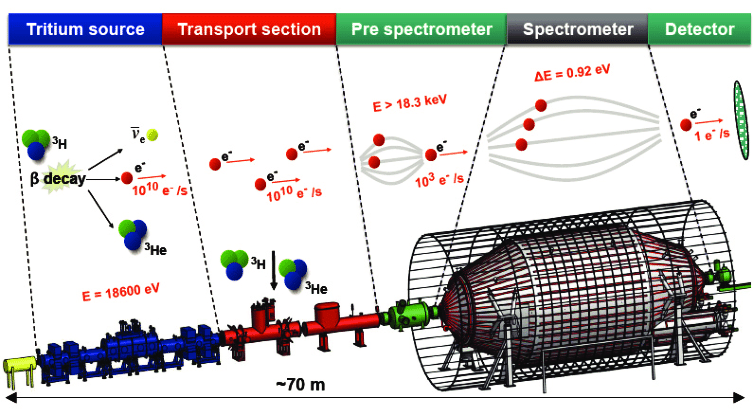
\includegraphics[width = \hugefigwidth]{figures-chap2/Schematics-of-the-Katrin-experiment.png}
    \caption[Schematic of the \gls{katrin} detector.]{Schematic of the \gls{katrin} detector \cite{KATRIN_detector_figure}.}
    \label{fig:katrin_detector}
\end{figure}

\paragraph{Neutrinoless Double Beta Decay}
Assuming that neutrinos are Majorana in nature, neutrinoless double beta decay (0$\nu\beta\beta$) should be an observable process in certain nuclei. The half-life, $T^{0\nu}$, of nuclei undergoing $0\nu\beta\beta$ is given by, 

\begin{equation}
    [T^{0\nu}]^{-1} = G^{0\nu} \cdot |M^{0\nu}|^2 \cdot \langle m_{\beta\beta}\rangle^2,
\end{equation}
where, $G^{0\nu}$, is the phase space factor, $M^{0\nu}$, is the matrix element and $\langle m_{\beta\beta}\rangle = \sum_i U^2_{ei}m_i$, which is the effective Majorana neutrino mass. Both $G^{0\nu}$ and $M^{0\nu}$ depend on the nucleus that undergoes the decay. Therefore, measuring the half-life of a $0\nu\beta\beta$ decay process gives a measure of the effective neutrino mass. 

Some of the most stringent limits on the effective neutrino mass are provided by the KamLAND-Zen experiment. As of yet no $0\nu\beta\beta$ has been observed and a lower bound on the half-life of $2.3 \times 10^{26}$ years at a 90\% confidence level which equates to an upper limit on the effective Majorana neutrino mass of 36 -- 156 meV, depending on the model of the nuclear matrix element \cite{kamlandZen}.

\paragraph{Cosmological Constraints}
A number of cosmological observations have put upper bounds on the neutrino mass. Some of the most stringent constraints come from the \textit{Planck} collaboration which measured temperature anisotropies in the cosmic microwave background \cite{PDG_2022}\cite{planck_2018}. 

By combining \textit{Planck} data with that from baryon acoustic oscillations (BAO) and Type Ia supernovae the total neutrino mass, $\sum m_\nu = m_1 + m_2 + m_3$, may be constrained to have an upper mass limit as low as 0.11 eV at the 95\% confidence level \cite{PDG_2022}\cite{planck_2018}.

\subsection{Neutrino Oscillations}\label{subsec:Neutrino Oscillations}

Another unique property of neutrinos are their ability to oscillate. That is, the neutrino flavour may change as it propagates. This phenomenon was first proposed by Pontecorvo in 1957 \cite{Pontecorvo}. In the following years, this work was built upon by Maki, Nakagawa, Sakata and Pontecorvo himself \cite{MNS_oscillations}. 

\subsubsection{3 Flavour Oscillation Phenomenology}

Neutrino oscillations is one of the key topics in the field and this thesis. The remainder of this section will discuss the theory of neutrino oscillations in both vacuum and in matter. The three flavour states (\nue, \numu, \nutau) have already been established,
but it is expected that the neutrino mass states \mbox{(\nuone, \nutwo, \nuthree)} are distinct in order to explain neutrino oscillations. The flavour eigenstate of a neutrino is what is observed, however, each flavour state is a superposition of the three mass states. As a neutrino propagates, the relative phase between the mass states is continuously changing. When a neutrino then interacts, the mass states may have a relative phase that is different to that when the neutrino was created. At the point of interaction, the flavour superposition will then collapse into a single flavour and this is what is then detected. This is the mechanism which allows neutrino flavours to oscillate. 

\paragraph{Oscillations in Vacuum}



The transformation between the flavour and mass states is expressed as
\begin{equation}\label{eqn:state transformation}
    \ket{\nu_\alpha} = \sum_k U^*_{\alpha k} \ket{\nu_k},
\end{equation}
where $\alpha$ $\in$ (e, $\mu$, $\tau$), k $\in$ (1, 2, 3) and \textit{U} is a unitary matrix. In the case of three flavour neutrino oscillations, \textit{U}, is known as the \gls{pmns} mixing matrix which is a $3 \times 3$ matrix representing the three different states \cite{Fundamentals_of_Neutrino_Physics_and_Astrophysics}. The \gls{pmns} matrix is parameterised in terms of three mixing angles ($\theta_{12}, \theta_{13}, \theta_{23}$) and a single physical \gls{cp} violating phase, \textit{$\Kronecker_{cp}$}\footnote{Here we are assuming that neutrinos are Dirac particles. If they are Majorana particles the \gls{pmns} matrix would have two additional phases as described in \SectionRef{subsubsec:CP_violation}.}, as
\begin{equation}
\begin{split}
U &= 
\begin{pmatrix}
U_{e1} & U_{e2} & U_{e3} \\
U_{\mu1} & U_{\mu2} & U_{\mu3}  \\
U_{\tau1} & U_{\tau2} & U_{\tau3}
\end{pmatrix} \\
&=
\begin{pmatrix}
1 & 0 & 0 \\
0 & c_{23} & s_{23}  \\
0 & -s_{23} & c_{23}
\end{pmatrix}
\begin{pmatrix}
c_{13} & 0 & s_{13}e^{-i\delta_{cp}} \\
0 & 1 & 0  \\
-s_{13}e^{i\delta_{cp}} & 0 & c_{13}
\end{pmatrix}
\begin{pmatrix}
c_{12} & s_{12} & 0 \\
-s_{12} & c_{12} & 0  \\
0 & 0 & 1
\end{pmatrix}
\end{split}
\end{equation}
where $c_{kj} = \cos{\theta_{kj}}$, $s_{kj} = \sin{\theta_{kj}}$ and the other 5 phases of the unitary matrix have been absorbed by rephasing the lepton fields. 

The time-dependent Schr{\"o}dinger equation is given by
\begin{equation} \label{eqn:t.d. schrodinger}
    i \dByd{}{t}\ket{\nu_{k}(t)} = H \ket{\nu_{k}(t)},
\end{equation}
and since neutrino mass states are eigenstates of the Hamiltonian, \textit{H},  it follows that the solution to \EquationRef{eqn:t.d. schrodinger} is given by a plane wave solution 
\begin{equation}\label{eqn:plane wave soln}
    \ket{\nu_{k}(t)} = e^{-iE_{k}t} \ket{\nu_{k}}.
\end{equation}
The amplitude of a transition, $A_{\nu_\alpha \rightarrow \nu_\beta}(t)$, is defined as the projection of the final state onto the initial state, so for flavour oscillations, the amplitude is given by
\begin{equation}
    A_{\nu_\alpha \rightarrow \nu_\beta}(t) \isdefinedas \braket{\nu_\beta|\nu_\alpha(t)}.
\end{equation}
The probability of transition, $P_{\nu_\alpha \rightarrow \nu_\beta}(t)$, is then given by the absolute square of the amplitude
\begin{equation}
    P_{\nu_\alpha \rightarrow \nu_\beta}(t) = |A_{\nu_\alpha \rightarrow \nu_\beta}(t)|^2.
\end{equation}
It follows from \EquationRef{eqn:state transformation} and \EquationRef{eqn:plane wave soln} that
\begin{equation}
    \ket{\nu_\alpha(t)} = \sum_k U^*_{\alpha k} e^{-iE_kt}\ket{\nu_k}
\end{equation}
and that the transition amplitude is given by
\begin{equation}
    A_{\nu_\alpha \rightarrow \nu_\beta}(t) = \sum_k U^*_{\alpha k} U_{\beta k} e^{-iE_kt}
\end{equation}
where the fact that $\braket{\nu_j|\nu_k} = \Kronecker_{jk}$ has been used since the mass eigenstates are orthonormal. It then follows that the oscillation probability is given by
\begin{equation}
    P_{\nu_\alpha \rightarrow \nu_\beta}(t) = \sum_{k,j} U^*_{\alpha k} U_{\beta k} U_{\alpha j} U^*_{\beta j} e^{-i(E_k-E_j)t}.
\end{equation}
Under the assumption that neutrinos are relativistic, the mass state energy, $E_k$, may be expressed in terms of the neutrino energy, \textit{E},
\begin{equation}
    E_k = \sqrt{|\Vec{p}|^2 + m_k^2} \simeq E + \frac{m_k^2}{2E}.
\end{equation}
By noting that the mass splitting, $\Delta m^2_{kj}$, is defined as 
\begin{equation}
    \Delta m^2_{kj} = m_k^2 - m_j^2
\end{equation}
and that for highly relativistic particles $t \approx L$, where \textit{L} is known as the baseline (i.e. the distance the neutrino has travelled), the oscillation probability may be written as 
\begin{equation}
     P_{\nu_\alpha \rightarrow \nu_\beta}(L,E) = \sum_{k,j} U^*_{\alpha k} U_{\beta k} U_{\alpha j} U^*_{\beta j} e^{-i\frac{\Delta m^2_{kj}L}{2E}}.
\end{equation}
It should be noted that what neutrino experiments probe is the mass splitting and not the absolute neutrino masses. Finally, for the special case where only two neutrinos contribute to mixing in a non-negligible way, the oscillation probability may be simplified to
\begin{comment}
\begin{equation}
\begin{split}
    P_{\nu_\alpha \rightarrow \nu_\beta} &= \sin^2(2\theta)sin^2(\frac{\Delta m^2L}{4E}), \ \ \ \ \nu_\alpha \neq \nu_\beta   \\
    P_{\nu_\alpha \rightarrow \nu_\alpha} &= 1 - P_{\nu_\alpha \rightarrow \nu_\beta},
\end{split}
\end{equation}
\end{comment}
\begin{equation}
  P_{\nu_\alpha \rightarrow \nu_\beta}=\begin{cases}
    \sin^2(2\theta)\sin^2{(\frac{\Delta m^2L}{4E})}, & \nu_\alpha \neq \nu_\beta \\
    1 - \sin^2(2\theta)\sin^2{(\frac{\Delta m^2L}{4E})}, & \nu_{\alpha} = \nu_{\beta},
  \end{cases}
  \label{eqn:osc_probability}
\end{equation}
where the mixing matrix has been reduced to a rotation matrix \cite{Fundamentals_of_Neutrino_Physics_and_Astrophysics}. 

\paragraph{Oscillations in Matter}

The neutrino oscillations discussed so far have assumed that the neutrinos are propagating in a vacuum. It was shown by Wolfenstein that neutrinos propagating in matter experience a potential due to coherent forward scattering with the electrons and nucleons \cite{Wolfenstein}. This potential may be thought of as an effect similar to the index of refraction in a material \cite{Fundamentals_of_Neutrino_Physics_and_Astrophysics}. Both \gls{cc} and \gls{nc} scattering may occur, however, \gls{cc} scattering may only occur for electron neutrinos whereas \gls{nc} scattering may occur for all active neutrino flavours equally. The total Hamiltonian for neutrinos propagating in matter, $H_T$, is, therefore, the vacuum Hamiltonian as seen in \EquationRef{eqn:t.d. schrodinger} plus the Hamiltonian due to the additional potential from matter effects, $H_m$. That is 
\begin{equation}
    H_T = H + H_m \text{ \hspace{1cm} with, } \begin{split}
        & H\ket{\nu_k} = E_k\ket{\nu_k} \\
        & H_m\ket{\nu_k} = V_m\ket{\nu_k},
    \end{split}
\end{equation} 
where $V_m$ is the effective potential the neutrinos are subjected to \cite{Fundamentals_of_Neutrino_Physics_and_Astrophysics}. In the three neutrino mass basis,
\begin{equation}
H_T = \frac{1}{2E} 
\begin{pmatrix}
m_1^2 & 0 & 0 \\
0 & m_2^2 & 0 \\
0 & 0 & m_3^2
\end{pmatrix}
+ U^\dag
\begin{pmatrix}
V_e & 0 & 0 \\
0 & 0 & 0 \\
0 & 0 & 0
\end{pmatrix}
U,
\end{equation}
where $V_e$ is the effective potential due to \gls{cc} scattering. It may be shown that 
\begin{equation}
    V_e = \pm \sqrt{2}G_Fn_e,
\end{equation}
where the positive value is used for neutrinos and the negative value for antineutrinos, $G_F$ is the Fermi constant and $n_e$ is the electron density in the medium.
The \gls{nc} component is omitted since it contributes equally to all neutrino flavours and therefore has no impact on the oscillation probability \cite{PDG_2022}. 

If only two neutrino species are considered, the mass splitting in matter, $\Delta m^2_m$, is given by 
\begin{equation}
    \Delta m_m^2 = m_{2m}^2 - m_{1m}^2 = \Delta m^2 \sqrt{(\cos{2\theta} - A/\Delta m^2)^2 + \sin^2{2\theta}},
\end{equation}
and the mixing angle in matter, $\theta_m$, is given by
\begin{equation}
    \tan{2\theta_m} = \frac{\sin{2\theta}}{\cos{2\theta} - A/\Delta m^2},
    \label{eqn:matter_mixing_angle}
\end{equation}
where $\Delta m^2$ and $\theta$ are the vacuum mass splitting and vacuum mixing angle respectively and $A \equiv 2EV_e$. The oscillation probability is the same as is shown in \EquationRef{eqn:osc_probability}, but substituting in the relevant matter mixing angle and mass splitting instead of the vacuum values. It should be noted that if $\theta = 0$, then $\theta_m = 0$, which means that oscillations in matter can only occur if oscillations in a vacuum are possible. Furthermore, if $A = \Delta m^2\cos{2\theta}$, \EquationRef{eqn:matter_mixing_angle} diverges. This critical value of \textit{A} is known as the \gls{msw} resonance and corresponds to $\theta_m = \pi/4$, which means that the oscillation probability is maximal. Therefore, for any non-zero vacuum oscillation probability, there exists a value of $A$ where the matter oscillation probability is a 100\% \cite{PDG_2022}. 

\subsubsection{3 Flavour Oscillation Experimental Results}

One of the first experimental results to eventually be explained by neutrino oscillations was the Homestake experiment. This was an experiment in the 1960s that was designed to count the number of solar neutrinos. The crux of the experiment was to fill an underground tank with dry-cleaning fluid (perchloroethylene) since it contains chlorine. The solar neutrinos would be detected by inverse beta decay via
\begin{equation}
    ^{37}Cl + \nue \longrightarrow {^{37}Ar} + \electron,
\end{equation}
where the argon would be extracted and counted as it decayed. From this, the number of interacting electron neutrinos was determined, however, this number was consistently about a third of the number expected by solar predictions. This inconsistency was later dubbed the \textit{Solar Neutrino Problem} \cite{Homestake}.

The ratio of muon to electron neutrinos produced in the atmosphere from the decay of pions and muons was also studied. The predicted rate of neutrinos in the atmosphere was thought to be well understood, however a number of experiments, the most notable of which, \Gls{sk}, all observed ratios significantly below the expected value. This indicated a deficit in the observed muon neutrinos or an excess in electron neutrinos (or both). Mirroring the solar neutrino problem, these observations were dubbed the \textit{Atmospheric Neutrino Anomaly} \cite{Atmospheric_anomaly}.

The \gls{sk} detector consists of a tank of 50,000 tons of pure water. Neutrino interactions with either electrons or nuclei from the water may result in Cherenkov light that is detected by \glspl{pmt} surrounding the detector. In addition to measuring the ratio of atmospheric neutrinos, \Gls{sk} was also able to measure the zenith angle of the incoming neutrinos. This allowed the observed and predicted number of neutrinos to be compared as a function of the zenith angle. It was noted that the number of electron neutrinos agreed reasonably well with the expected value across all angles whereas for low-energy muon neutrinos there was a deficit of events for all angles and for high-energy muons, there was a deficit of events for zenith angles corresponding to large distances travelled (e.g. neutrinos which travelled through the earth and into the detector from below). The observed rate of high energy muons at angles corresponding to travelling directly down from the atmosphere to the detector agreed with predicted values \cite{SuperK_neutrino_oscillations}. 

The results published by \gls{sk} in 1998 allowed the atmospheric neutrino anomaly to be reconciled with neutrino oscillations and was the first time neutrino oscillations were confirmed to have been observed \cite{SuperK_neutrino_oscillations}. Shortly after, in 2001, the \Gls{sno} resolved the solar neutrino problem by again explaining the deficit in observed electron neutrinos as a result of neutrino oscillations. The \gls{sno} detector was designed with the intention of being able to measure the total neutrino flux (the sum of all three flavours) and the electron neutrino flux in isolation. The detector consisted of a tank of heavy water. Solar neutrinos have sufficient energy to interact via \gls{nc} interactions with the deuterium in the heavy water regardless of neutrino flavour,
\begin{equation}
    \nu + d \longrightarrow \nu + p + n.
\end{equation}
Neutrinos of any flavour may also interact via \gls{es},
\begin{equation}
    \nu + \electron \longrightarrow \nu + \electron.
\end{equation}
\gls{es} interactions are subdivided into \gls{cc} and \gls{nc} components, but since only \nue's are above the threshold energy for \gls{cc} interactions, there is no \gls{cc} component for \numu or \nutau. Therefore, all active neutrino flavours contribute equally to the \gls{nc} \gls{es} flux, but the flux of \nue's is enhanced due to also having a \gls{cc} component \cite{SNO_ES}. Finally, only electron neutrinos may interact via \gls{cc},
\begin{equation}
    \nue + d \longrightarrow p + p + \electron,
\end{equation}
therefore this channel only measured the flux of \nue. Confirmation that the flux of \nue was less than the flux from the \gls{nc} or \gls{es} channels coupled with the fact that the \nue flux was in agreement with previous solar neutrino experiments was sufficient to resolve the solar neutrino problem \cite{SNO_solar_neutrinos}.

It is understood from oscillation experiments that $\Delta m_{21}^2$, known as the solar mass splitting, is equal to $\sim 7.5 \times 10^{-5}$ eV$^2$ and that $|\Delta m_{31}^2|$, known as the atmospheric mass splitting, is equal to $\sim2.4 \times 10^{-3}$ eV$^2$. The sign of the atmospheric mass splitting is, however, unknown i.e. it is an open question whether $m_3$ is the heaviest or the lightest neutrino mass state. This leads to two possibilities, the so-called \textit{normal hierarchy} where the neutrino mass states increase from $m_{1 \rightarrow 2 \rightarrow 3}$ or the \textit{inverted hierarchy} where the mass states increase from $m_{3 \rightarrow 1 \rightarrow 2}$. This is shown graphically in \FigureRef{fig:mass_hierarchy}. 

A key feature of \EquationRef{eqn:matter_mixing_angle} is that the matter mixing angle depends on the sign of $\Delta m^2$. This is not the case for vacuum oscillations. The sign of $\Delta m^2_{21}$ was determined using the matter effect by comparing day and night solar neutrino interactions in \gls{sk}. An asymmetry in the day/night flux of \nue's was observed because during the night, neutrinos travel through the earth and thus the matter effect becomes relevant whereas during the day, the matter that neutrinos traverse is negligible. Therefore, unlike vacuum oscillations, matter oscillations may be used to determine the neutrino mass hierarchy within a 2-flavour approximation.

\begin{comment}
In order to determine the mass hierarchy using vacuum oscillations, the full 3-flavour oscillation probability must be used with the requirement that a given experiment is sensitive to both $\Delta m^2_{21}$ and $\Delta m^2_{31}$ \cite{mass_hierarchy_discussion}\cite{Neutrino_Mass_Hierarchy_Vacuum_Oscillations_and_Vanishing_Ue3}.
\end{comment}

The nature of the neutrino hierarchy has major impacts on several areas. Within the inverted hierarchy, there is a lower bound on the Majorana mass of the electron neutrino mass. If neutrinoless double beta decay experiments can put bounds on the neutrino mass below this, the inverted hierarchy may be ruled out (under the assumption that neutrinos are Majorana in nature). Alternatively, if the inverted hierarchy is realised, neutrinoless double beta decay experiments are promising ways to determine whether neutrinos are Majorana particles or not. There are also a number of theories which predict either the normal or inverted hierarchy, so determining the hierarchy will be a strong motivator in determining the credibility of a given theory \cite{mass_hierarchy}.

\begin{figure}[h!]
    \centering
    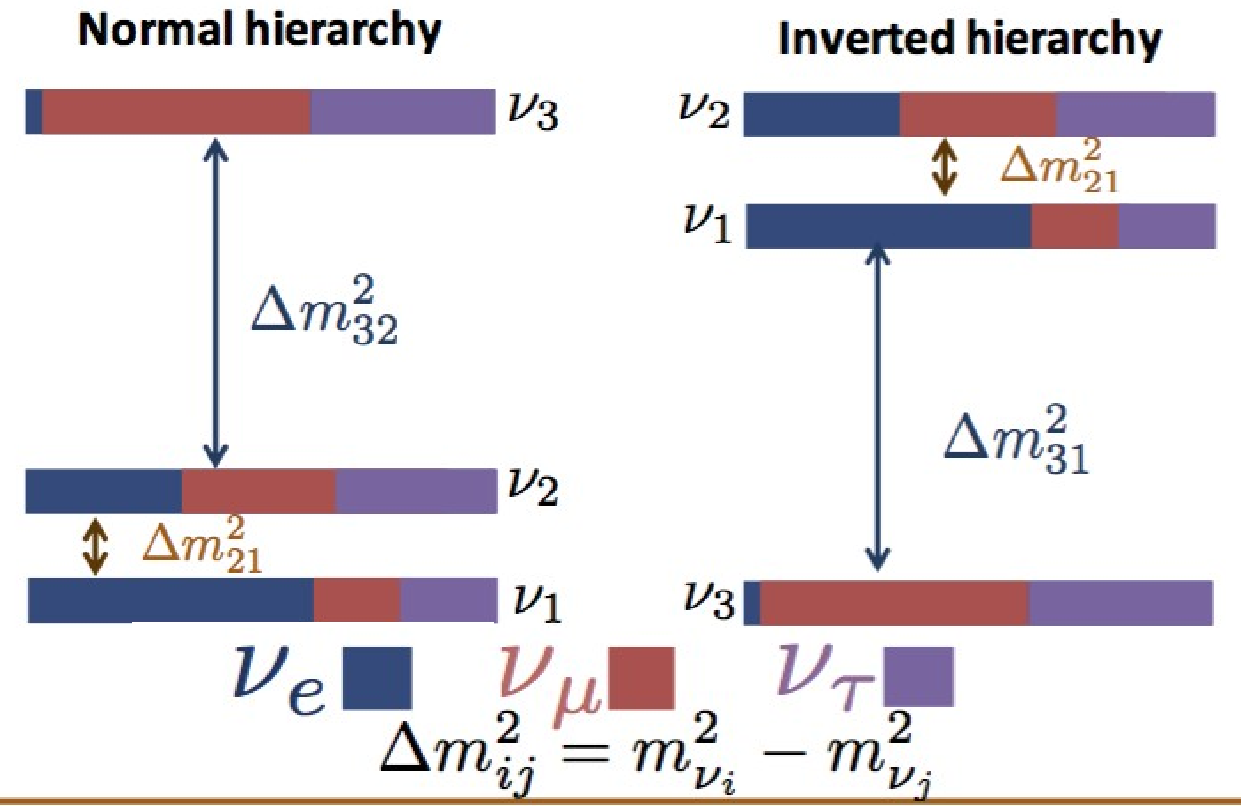
\includegraphics[width = \largefigwidth]{figures-chap2/mass_hierarchy-crop.pdf}
    \caption[Neutrino hierarchy.]{Diagrammatic representation of the normal hierarchy (left) and the inverted hierarchy (right). The flavour contributions to each mass state are illustrated by the different colours \cite{mass_hierarchy_image_2}.}
    \label{fig:mass_hierarchy}
\end{figure}



\newpage
The best fit values for oscillation parameters and the \gls{cp} violating phase from a 3-flavour neutrino framework are shown in \TableRef{table:Best fit params} for both the normal and inverted hierarchy \footnote{The factor of 2 in the argument of $\sin^2{2\theta}$ is sometimes absorbed into the mixing angle as is the case for example in Figures \ref{fig:theta_21_deltamsq_21_best_fit}--\ref{fig:t2k_nova_CP}.}. The numbers have been provided by the 2020 edition of the \gls{pdg} collaboration \cite{PDG_2020}. Some of the experiments that have determined the oscillation parameters are discussed below. 

\begin{table}[h!]
\begin{tabular}{l ll}
\multicolumn{1}{c}{\multirow{2}{*}{Parameter}} & \multicolumn{2}{c}{Best Fit}                                                                           \\
\multicolumn{1}{c}{} & \multicolumn{1}{c}{Normal Hierarchy} & \multicolumn{1}{c}{Inverted Hierarchy}   \\  \hline
$sin^22\theta_{12}$ & \multicolumn{1}{r}{$0.307\pm0.013$}                                        & \multicolumn{1}{r}{$0.307\pm0.013$}  \\
$sin^22\theta_{13}$ & \multicolumn{1}{r}{$(2.20\pm0.07) \times 10^{-2}$}                         & \multicolumn{1}{r}{$(2.20\pm0.07) \times 10^{-2}$} \\
$sin^22\theta_{23}$ & \multicolumn{1}{r}{$0.546\pm 0.021$}                                       & \multicolumn{1}{r}{0.539 \pm 0.022}    \\
$\Delta m^2_{21}$   & \multicolumn{1}{r}{$(7.53\pm0.18) \times 10^{-5} \text{ eV}^2$}                     & \multicolumn{1}{r}{$(7.53\pm0.18) \times 10^{-5} \text{ eV}^2$}   \\
$\Delta m^2_{32}$   & \multicolumn{1}{r}{$(2.453\pm0.033) \times 10^{-3} \text{ eV}^2$} & $(-2.536 \pm 0.034) \times 10^{-3} \text{ eV}^2$ \\
$\delta_{CP}$       & \multicolumn{1}{r}{$1.36^{+0.20}_{-0.16} \pi$ rad}                         &  \multicolumn{1}{r}{$1.36^{+0.20}_{-0.16} \pi$ rad} \\  
\end{tabular}
\caption[3-flavour neutrino best fit values.]{The best fit values for 3-flavour neutrino oscillation parameters from the 2020 \gls{pdg} \cite{PDG_2020}.}
\label{table:Best fit params}
\end{table}

\newpage

\paragraph{$\Delta m^2_{21}$ and $sin^22\theta_{12}$}
The $\Delta m^2_{21}$ and $sin^22\theta_{12}$ parameter values are determined from the solar neutrino experiments, Homestake, GALLEX/GNO, SAGE, Borexino, phases I-IV of \gls{sk} and the three phases of \gls{sno} \cite{Gallex_reanalysis}\cite{Measurement_of_the_Solar_Electron_Neutrino_Flux_with_the_Homestake_Chlorine_Detector}\cite{Measurement_of_the_solar_neutrino_capture_rate_with_gallium_metal}\cite{Precision_measurement_of_the_7Be_solar_neutrino_interaction_rate_in_Borexino}\cite{Final_results_of_Borexino_PhaseI_on_low_energy_solar_neutrino_spectroscopy} \cite{Solar_neutrino_measurements_in_Super-Kamiokande-I}\cite{Solar_neutrino_measurements_in_Super-Kamiokande-II}\cite{Solar_neutrino_results_in_Super-Kamiokande-III}\cite{8B_solar_neutrino_spectrum_measurement_using_Super-Kamiokande_IV}\cite{Combined_Analysis_of_all_Three_Phases_of_Solar_Neutrino_Data_from_the_Sudbury_Neutrino_Observatory}. The relevant standard solar model used in the combined analysis is AGSS09 \cite{AGSS09}. In addition to the solar experiments, the KamLAND experiment, which detected neutrinos from a number of nuclear reactors over a long baseline ($\sim180$ km), also measured the solar mass splitting and mixing angles. \cite{Precision_Measurement_of_Neutrino_Oscillation_Parameters_with_KamLAND}\cite{Constraints_on_theta13_from_A_Three_Flavor_Oscillation_Analysis_of_Reactor_Antineutrinos_at_KamLAND}\cite{Reactor_On-Off_Antineutrino_Measurement_with_KamLAND} A global fit of the solar experiments and the KamLand results are shown in \FigureRef{fig:theta_21_deltamsq_21_best_fit} along with a combined fit of the two \cite{2020_global_reassessment_of_the_neutrino_oscillation_picture}. The best fit point from the allowed region of the solar experiments is highly disfavoured by the KamLAND experiment, however, the 99\% confidence level allowed regions do overlap. 

\begin{figure}[h!]
    \centering
    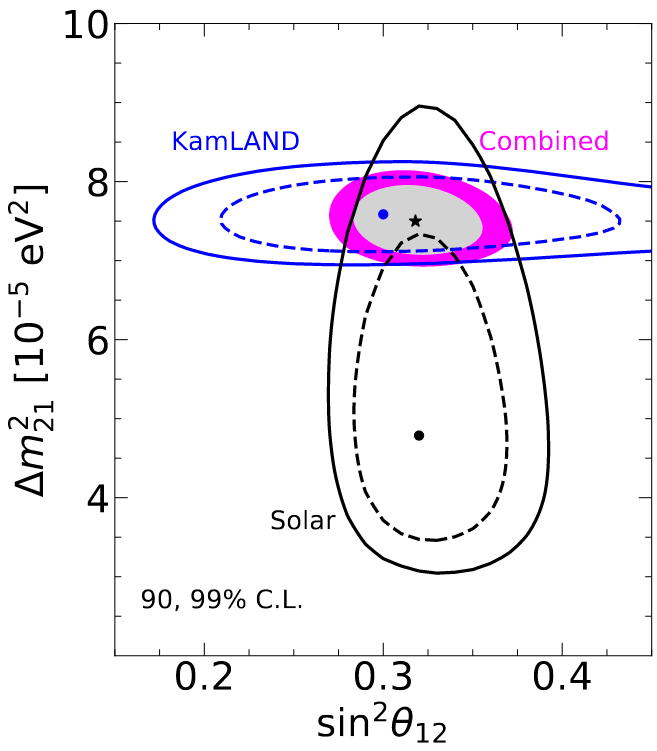
\includegraphics[width = \smallfigwidth]{figures-chap2/theta_12.png}
    \caption[A global fit of the allowed region in $\sin^2{\theta_{12}}$ -- $\Delta m^2_{21}$ space from solar experiments and the KamLAND experiment.]{A global fit of the allowed region in $\sin^2{\theta_{12}}$ -- $\Delta m^2_{21}$ space from solar experiments, the KamLAND experiment and a combination of the two. The relevant best fit points are also shown
    \cite{2020_global_reassessment_of_the_neutrino_oscillation_picture}.}
    \label{fig:theta_21_deltamsq_21_best_fit}
\end{figure}


\paragraph{$\Delta m^2_{31}$ and $sin^22\theta_{13}$}
Parameters $\Delta m^2_{31}$ and $sin^22\theta_{13}$ may again be determined from reactor neutrino experiments, but with baselines considerably shorter than that of KamLAND. The \gls{reno} experiment consists of two identical detectors which detect electron antineutrinos from 6 reactors. The 6 reactors are part of a linear 1.3 km array with equal spacing between each reactor and the two \gls{reno} detectors are 294 m and 1383 m either side of the centre of the reactor array. The \nuebar's are detected in a liquid scintillator doped with gadolinium via inverse beta decay \cite{Measurement_of_Reactor_Antineutrino_Oscillation_Amplitude_and_Frequency_at_RENO}. After a 2900 day data taking period, \gls{reno} determined that the mixing angle, $\sin^2{2\theta_{13}} = 0.0892 \pm 0.0063$ and that the mass splitting, $|\Delta m^2_{ee}| = (2.74 \pm 0.12) \times 10^{-3}$ eV$^2$, where $|\Delta m^2_{ee}| = \cos^2{\theta_{12}}\Delta m^2_{31} + \sin^2{\theta_{12}}\Delta m^2_{32}$ \cite{RENO_2020}. 

The Daya Bay experiment consists of eight antineutrino detectors which measure the oscillation probability from the antineutrinos produced from the Daya Bay nuclear plant. There are two associated near experimental halls each of which houses two of the detectors and one far experimental hall which houses the other four detectors. The near detectors have a baseline of $\sim0.3$--1.3 km whereas the far detectors have a baseline of $\sim1.5$--1.9 km \cite{2020_global_reassessment_of_the_neutrino_oscillation_picture}. The detectors consist of a cylindrical gadolinium-doped liquid scintillator target which is surrounded by undoped liquid scintillator which is in turn surrounded by \glspl{pmt}. After 1958 days of data taking, Daya Bay determined that the mixing angle, $\sin^2{2\theta_{13}} = 0.0856 \pm 0.0029$ and that the mass splitting, $|\Delta m^2_{ee}| = (2.522^{+0.068}_{-0.070}) \times 10^{-3}$ eV$^2$ \cite{Measurement_of_electron_antineutrino_oscillation_with_1958_days_of_operation_at_Daya_Bay}.

The allowed regions and best fit points from both \gls{reno} and Daya Bay are shown in \FigureRef{fig:Reno_Daya_Bay} for both the normal and inverted hierarchy, but since neither experiment is sensitive to the mass ordering the results are essentially the same. Much of the allowed parameters space is consistent between the two experiments \cite{2020_global_reassessment_of_the_neutrino_oscillation_picture}.

\begin{figure}
    \centering
    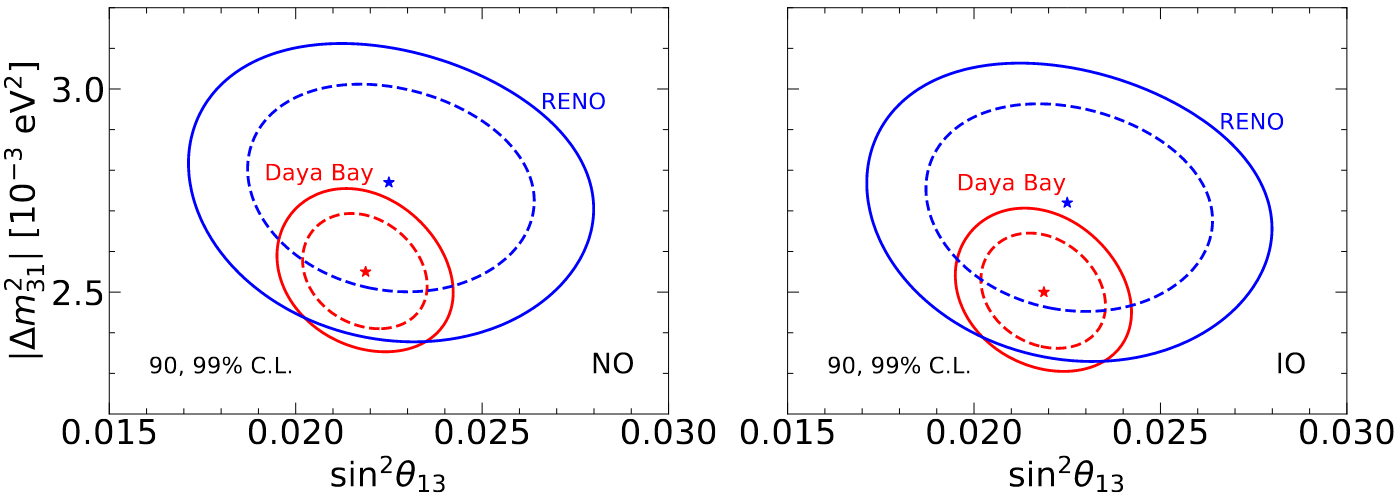
\includegraphics[width = \hugefigwidth]{figures-chap2/theta_13.png}
    \caption[Allowed regions in $\sin^2{\theta_{13}}$ -- $\Delta m^2_{31}$ space from the \gls{reno} and Daya Bay experiments.]{Allowed regions from a global analysis in $\sin^2{\theta_{13}}$ -- $\Delta m^2_{31}$ space from the \gls{reno} and Daya Bay experiments for the normal hierarchy (left) and the inverted hierarchy (right). The associated best fit points are also shown
    \cite{2020_global_reassessment_of_the_neutrino_oscillation_picture}.}
    \label{fig:Reno_Daya_Bay}
\end{figure}

\paragraph{$\Delta m^2_{31}$, $\sin^2{2\theta_{23}}$ and $\delta_{CP}$}
Both atmospheric neutrino experiments and accelerator neutrino experiments may be used to measure $\Delta m^2_{31}$ and $\sin^2{2\theta_{23}}$. Atmospheric experiments detect neutrinos resulting from cosmic rays interacting in the atmosphere which result in particle showers that produce a neutrino flux that is comprised mainly of $\overset{(-)}{\nu}_{\!\!\mu}$'s. Long baseline accelerator experiments typically utilise a semi-pure $\overset{(-)}{\nu}_{\!\!\mu}$ beam and measure $\overset{(-)}{\nu}_{\!\!\mu}$ disappearance as well as $\overset{(-)}{\nu}_{\!\!e}$ appearance. In addition to $\Delta m^2_{31}$ and $\theta_{23}$, accelerator experiments are sensitive to $\theta_{13}$ and $\delta_{CP}$ \cite{2020_global_reassessment_of_the_neutrino_oscillation_picture}. 


The \gls{sk} experiment measured both the \numu disappearance and \nue appearance channels using atmospheric neutrinos with the former providing most of the sensitivity to $\Delta m^2_{31}$ and $\theta_{23}$. It was determined that $\Delta m^2_{31} = 2.63^{+0.10}_{-0.21} \times 10^{-3}$ eV$^2$ for the normal hierarchy and that $\Delta m^2_{31} = 2.53^{+0.14}_{-0.08} \times 10^{-3}$ eV$^2$ for the inverted hierarchy. Within the normal hierarchy, it was determined that $\sin^2{2\theta_{23}} = 0.425^{+0.051}_{-0.034}$ in the first octant and $\sin^2{2\theta_{23}} = 0.588^{+0.030}_{-0.062}$ in the second octant and within the inverted hierarchy, it was determined that $\sin^2{2\theta_{23}} = 0.425^{+0.075}_{-0.027}$ in the first octant and $\sin^2{2\theta_{23}} = 0.575^{+0.034}_{-0.075}$ in the second octant \cite{Atmospheric_Neutrino_Oscillation_Analysis_With_Improved_Event_Reconstruction_in_Super_Kamiokande_IV}.

The IceCube Deep Core experiment, which consists of 5160 \glspl{pmt} located $\sim2$ km below the geographic South Pole recorded over $10^5$ atmospheric neutrinos per year via Cherenkov radiation in the ice. Following 3 years of data taking where both track and shower like events where observed, it was determined that the mixing angle, $\sin^2{2\theta_{23}} = 0.53^{+0.09}_{-0.12}$ and that the mass splitting, $|\Delta m^2_{31}| = 2.72^{+0.19}_{-0.20} \times 10^{-3}$ eV$^2$ \cite{Determining_neutrino_oscillation_parameters_from_atmospheric_muon_neutrino_disappearance_with_three_years_of_IceCube_DeepCore_data}. The allowed region from the global analysis of \gls{sk} and IceCube DeepCore are shown in \FigureRef{fig:sk_icecube} for both the normal and inverted hierarchy \cite{2020_global_reassessment_of_the_neutrino_oscillation_picture}.

\begin{figure}[h!]
    \centering
    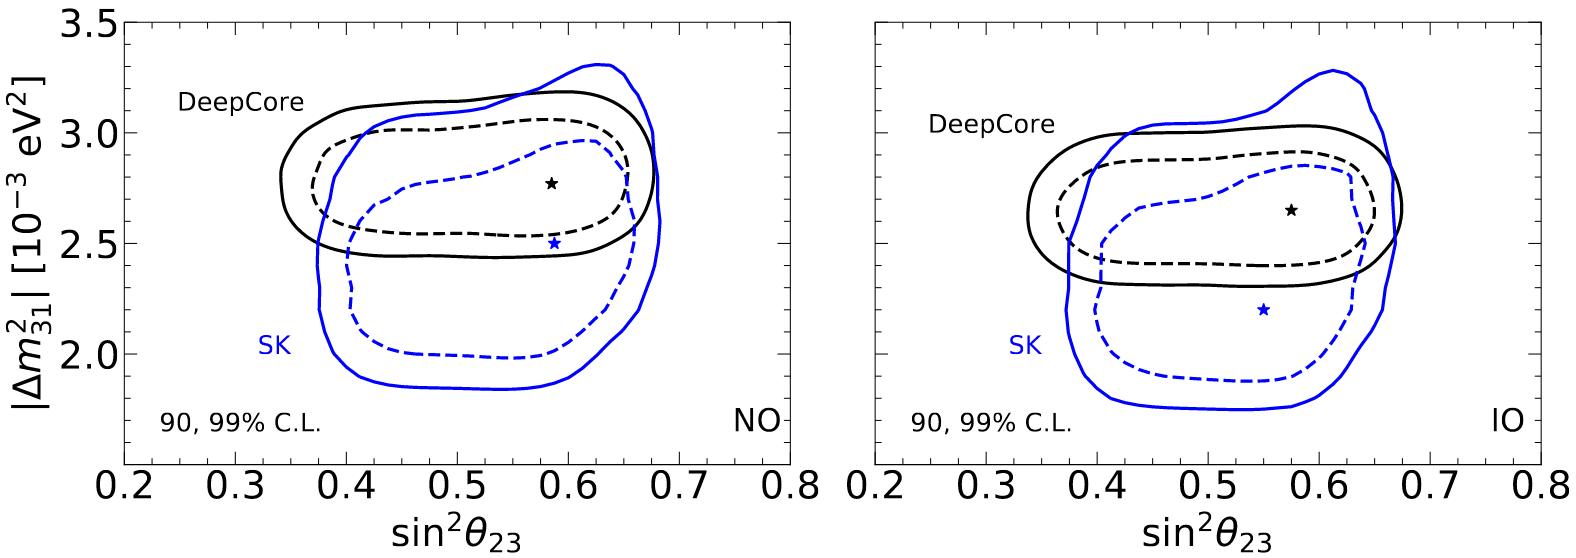
\includegraphics[width = \hugefigwidth]{figures-chap2/theta_23_2.png}   
    \caption[Allowed regions in $\sin^2{\theta_{23}}$ -- $\Delta m^2_{31}$ space from the \gls{sk} and IceCube DeepCore experiments.]{Allowed regions from a global analysis in $\sin^2{\theta_{23}}$ -- $\Delta m^2_{31}$ space from the \gls{sk} and IceCube experiments for the normal hierarchy (left) and the inverted hierarchy (right). The associated best fit points are also shown \cite{2020_global_reassessment_of_the_neutrino_oscillation_picture}.}
    \label{fig:sk_icecube}
\end{figure}

The \gls{t2k} experiment observed events from a beam exposure of $1.97 \times 10^{21}$ \gls{pot} in neutrino mode and $1.63 \times 10^{21}$ \gls{pot} in antineutrino mode. The neutrino beam is produced at the J-PARC facility and then travels 295 km to the \gls{sk} detector. There are also two near detectors as part of the \gls{t2k} experiment located at 280 m from the beam source, INGRID and ND280, which monitor the beam direction and stability and measure the flux of neutrinos respectively. 318 muon events and 137 antimuon events were observed as well as 94 electron events and 16 antielectron events. Additionally 14 electron events along with an electron from pion decays were observed \cite{T2K_2020}. Similarly, the NO$\nu$A experiment consists of a near detector and far detector located 1 km and 810 km from the beam source respectively and utilises the \gls{fermilab} NuMI neutrino beam. Both detectors are comprised of PVC cells containing liquid scintillator with the near detector having a mass of 290 tons whereas the far detector has a mass of 14,000 tons. NO$\nu$A observed 212 muon and 82 electron events from a beam exposure of $1.3.6 \times 10^{20}$ \gls{pot} whilst running in neutrino mode and 137 antimuon and 16 antielectron events from a beam exposure of $12.5 \times 10^{20}$ \gls{pot} whilst running in antineutrino mode \cite{New_constraints_on_oscillation_parameters_from_nue_and_numu_disappearance_in_the_NOvA_experiment}\cite{First_measurement_of_neutrino_oscillation_parameters_using_neutrinos_and_antineutrinos_by_NOvA}. The global analysis for the allowed region in $\sin^2{\theta_{23}}$ -- $\Delta m^2_{31}$ space (which assumes no prior on $\theta_{13}$) are shown in \FigureRef{fig:t2k_nova_minos_k2k} using data from \gls{t2k} and NO$\nu$A experiments as well as \gls{minos} and the K2K experiment for both the normal and inverted hierarchy  \cite{Measurement_of_Neutrino_and_Antineutrino_Oscillations_Using_Beam_and_Atmospheric_Data_in_MINOS}\cite{Electron_Neutrino_and_Antineutrino_Appearance_in_the_Full_MINOS_Data_Sample}\cite{K2K_experiment}. \FigureRef{fig:t2k_nova_CP} shows the allowed region in $\sin^2{\theta_{13}}$ -- $\delta_{CP}$ space from the global analysis using data from \gls{t2k} and NO$\nu$A. Results from the \gls{minos} and K2K experiments are not included as they are not sensitive to $\theta_{13}$ or $\delta_{CP}$ \cite{2020_global_reassessment_of_the_neutrino_oscillation_picture}. 

\begin{figure}[h!]
    \centering
    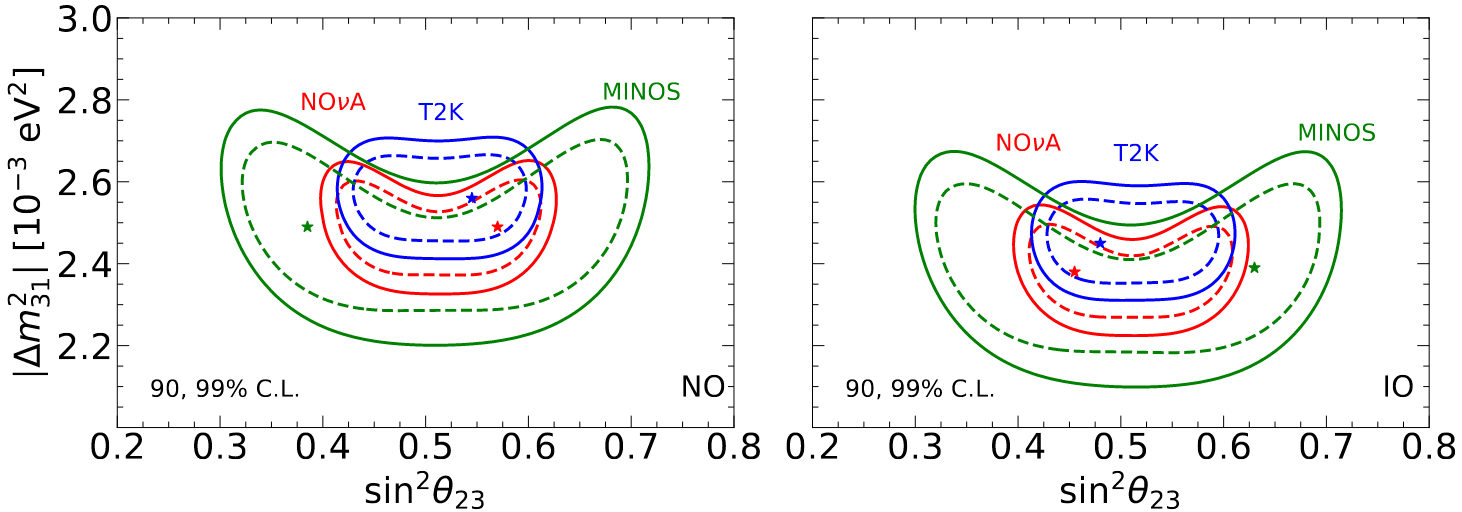
\includegraphics[width = \hugefigwidth]{figures-chap2/theta_23_1.png}   
    \caption[Allowed regions in $\sin^2{\theta_{23}}$ -- $\Delta m^2_{31}$ space from the \gls{t2k}, NO$\nu$A, \gls{minos} and K2K experiments.]{Allowed regions from a global analysis in $\sin^2{\theta_{23}}$ -- $\Delta m^2_{31}$ space from the \gls{t2k}, NO$\nu$A, \gls{minos} and K2K experiments for the normal hierarchy (left) and the inverted hierarchy (right). The associated best fit points are also shown
    \cite{2020_global_reassessment_of_the_neutrino_oscillation_picture}.}
    \label{fig:t2k_nova_minos_k2k}
\end{figure}

\begin{figure}[h!]
    \centering
    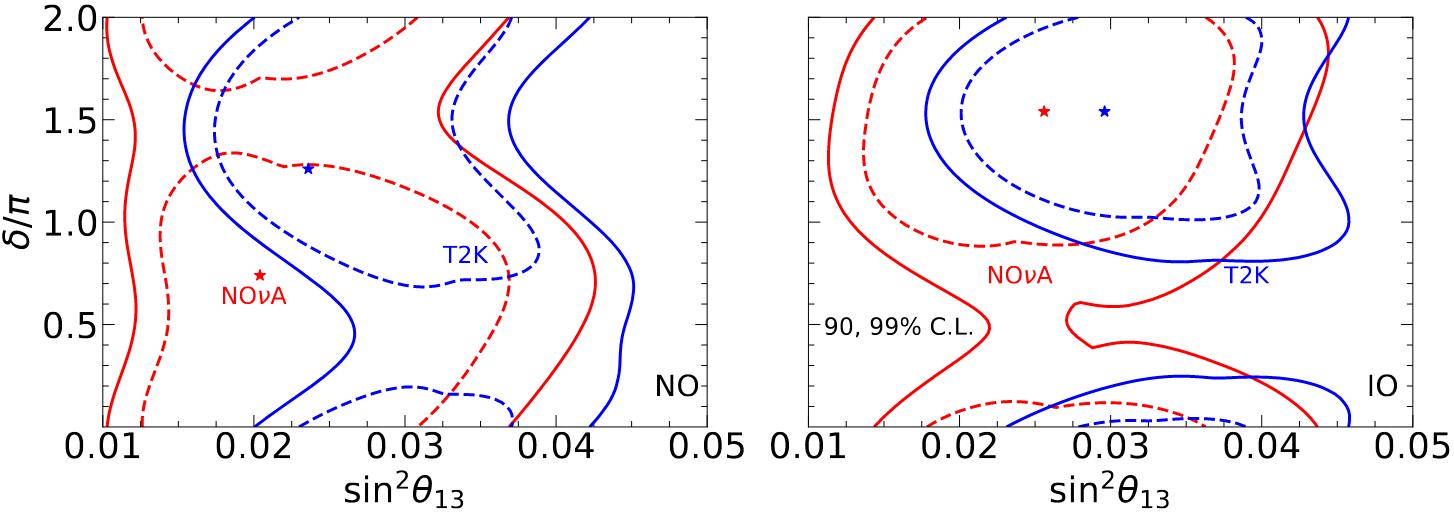
\includegraphics[width = \hugefigwidth]{figures-chap2/CP.png}
    \caption[Allowed regions in $\sin^2{\theta_{13}}$ -- $\delta_{CP}$ space from the \gls{t2k} and NO$\nu$A experiments.]{Allowed regions from a global analysis in $\sin^2{\theta_{13}}$ -- $\delta_{CP}$ space from the \gls{t2k} and NO$\nu$A experiments for the normal hierarchy (left) and the inverted hierarchy (right). The associated best fit points are also shown
    \cite{2020_global_reassessment_of_the_neutrino_oscillation_picture}.}
    \label{fig:t2k_nova_CP}
\end{figure}

\newpage
\subsubsection{Sterile Neutrino Oscillation Phenomenology}

An overview of the physics describing neutrino oscillations within the active sector was presented in \SectionRef{subsec:Neutrino Oscillations}. This approach may be extended to include an arbitrary number of additional neutrino states by expanding the \gls{pmns} matrix to include the desired number of sterile neutrinos

\begin{equation}
U_{sterile} = 
\begin{pmatrix}
U_{e1} & U_{e2} & U_{e3} & U_{e4} & \dots\\
U_{\mu1} & U_{\mu2} & U_{\mu3} & U_{\mu4} & \dots \\
U_{\tau1} & U_{\tau2} & U_{\tau3} & U_{\tau4} & \dots \\
U_{s1} & U_{s2} & U_{s3} & U_{s4} & \dots \\
\vdots & \vdots & \vdots & \vdots & \ddots \\
\end{pmatrix}.
\end{equation}
For simplicity, often only the special case with one sterile neutrino that is heavier than the three active neutrinos is considered. This is known as the $(3 + 1)$ neutrino framework which takes into account the three usual active neutrinos with the addition of one sterile neutrino. Within a $(3 + 1)$ framework and assuming that $\Delta m^2_{41} \gg |\Delta m^2_{31}|, \Delta m^2_{21}$, short baseline oscillation are well represented by the two flavour oscillation probability,

\begin{equation}
    P_{\nu_\alpha \rightarrow \nu_\beta} = \Kronecker_{\alpha \beta} -4|U_{\alpha \beta}|^2 (\Kronecker_{\alpha \beta} -|U_{\alpha \beta}|^2)\sin^2{\left(\frac{\Delta m^2_{41}L}{4E} \right)},
\label{eqn:sterile_osc_prob}
\end{equation}
where $\delta_{\alpha\beta}$ is the Kronecker delta between states $\alpha$ and $\beta$, $U_{\alpha \beta}$ are the relevant entries from the \gls{pmns} matrix and $\Delta m^2_{41}$ is the mass splitting involving the sterile neutrino state \cite{SBN_paper}. 

When performing a search for sterile neutrinos, typically there are three channels, one or more of which may be probed (plus their corresponding antineutrino variants). For each of these channels, the relevant \gls{pmns} matrix elements are parameterised in terms of mixing angles such that,
\begin{equation}
\centering
    &\text{\numu disappearance } (\numu \rightarrow \numu) &: \sin^2{2\thetamumu} &\isdefinedas 4|U_{\mu 4}|^2(1 - |U_{\mu 4}|^2) \label{eqn:sinsq2thmumu}\\
    &\text{\nue appearance } (\numu \rightarrow \nue) &: \sin^2{2\thetamue} &\isdefinedas 4|U_{\mu 4}|^2|U_{e4}|^2 \label{eqn:sinsq2thmue} \\
    &\text{\nue disappearance } (\nue \rightarrow \nue) &: \sin^2{2\thetaee} &\isdefinedas 4|U_{e 4}|^2(1 - |U_{e4}|^2).
    \label{eqn:sinsq2thee}
\end{equation}
It should be noted that \nue appearance depends on $U_{\mu 4}$ and $U_{e4}$, which \numu and \nue disappearance depend on respectively. The observation of \nue appearance would therefore automatically imply that \numu and \nue disappearance is also present. Additionally, this allows these parameters to be over-constrained \cite{SBN_paper}. The current global best fit values for the three mixing angles and the mass splitting term, $\Delta m^2_{41}$ are outlined in \TableRef{table:sterile_best_fit_params}.

\begin{table}[h!]
\begin{tabular}{c cc}
Oscillation Parameter        & \begin{tabular}[c]{@{}c@{}} Best Fit Value\end{tabular} \\ \hline

$\sin^2{2\theta_{\mu\mu}}$ & 0.07157      \\
$\sin^2{2\theta_{\mu e}}$ & 0.0009809      \\
$\sin^2{2\theta_{ee}}$ & 0.05310      \\
$\Delta m^2_{41}$ & 1.32 eV$^2$     \\

\end{tabular}
\caption[Best fit value for sterile oscillation parameters.]{The global best fit values for the $(3 + 1)$ sterile neutrino oscillation parameters \cite{Where_are_we_with_light_sterile_neutrinos}.}
\end{table}\label{table:sterile_best_fit_params}

\subsubsection{Sterile Neutrino Oscillation Experimental Motivation}\label{subchap:Motivation for Sterile Neutrinos}

\begin{comment}
\textcolor{red}{Other crap}
Cosmology: $N_{eff} = (3.046 + \Delta N_{eff})$
For any thermalised sterile neutrinos, $\Delta N_{eff} = 1, 2, 3 ...$
Measurements have $\Delta N_{eff} \sim 0$. 
So sterile neutrinos not thermalised.? Or at least suppressed
SBL steriles imply full thermalisation (why??) - so tension...
https://s3.cern.ch/inspire-prod-files-c/
c6eedeb5b3b604ca58f1a237e1b36f30
https://arxiv.org/pdf/1904.07108.pdf page 16
https://journals.aps.org/prd/pdf/10.1103/PhysRevD.104.123524
\end{comment}

There have been a number of experimental results which are not consistent with oscillations in a three-neutrino model. Most of these anomalous results can be explained by oscillations with one or more eV scale neutrinos pointing towards the existence of at least one light sterile neutrino. Experiments reporting these anomalous results include, \gls{lsnd} and \gls{miniboone} as well as data from reactor and gallium based experiments all of which are in tension with the null results reported from other experiments \cite{Where_are_we_with_light_sterile_neutrinos}. These results which are seemingly in favour of eV scale sterile neutrinos are discussed below along with the null results from \gls{karmen}, \gls{minos}, \gls{katrin}, \gls{t2k}, IceCube, \gls{microboone}, \gls{stereo}.

\paragraph{LSND}
The \gls{lsnd} experiment involved a close to 800 MeV proton beam which produced mainly $\pi^+$ and was designed to focus on the search for $\numubar \rightarrow \nuebar$ appearance where the \numubar's were a result from the decay of antimuons which in turn were produced from the \gls{dar} $\pi^+$. $\numu \rightarrow \nue$ oscillations were also studied resulting from \gls{dif} modes. The detector consisted of a tank filled with 167 tons of liquid scintillator (mineral oil) positioned 30~m from the neutrino beam source. An array of 1220 \glspl{pmt} were located on the inside of the tank and were used to detect both Cerenkov and scintillation light. Data was taken over a period of 6 years between 1993 and 1998. 

The electron selection was designed to minimise backgrounds from cosmic rays whilst still being able to identify electron events from neutrino interactions. For the $\numubar \rightarrow \nuebar$ oscillations, the energy range considered is 20--60 MeV, whereas for the $\numu \rightarrow \nue$ oscillations an energy range of 60--200 MeV was used. The minimum energy of 20 MeV was chosen because the $\beta$-decay of $^{12}$B resulting from the capture of $\mu^-$ on $^{12}$C in the target would lead to a significant background. The maximum energy of 200 MeV was chosen as above this there would be a significant background from $\pi^+ \rightarrow \positron + \nue$ decays compared to the oscillation signals. 

The \nuebar appearance signal was identified from the $\nuebar + p \rightarrow \positron + n$ reaction with the signature of the reaction being the energy of the \positron and the energy of a gamma as a result of neutron capture on a free proton. The \gls{lsnd} experiment observed an excess of \mbox{$87.96 \pm 22.46_{(stat)} \pm 6.0_{(syst)}$} events from $\nuebar + p \rightarrow \positron + n$ reactions which corresponds to a 3.8$\sigma$ excess which is shown in \FigureRef{fig:LSND excess}. The $\numu \rightarrow \nue$ did not show a clear excess in events, but was still consistent with the $\numubar \rightarrow \nuebar$ signal \cite{LSND_excess}. This was the first experiment to point towards the existence of an eV-scale neutrino. 



\begin{figure}[h!]
    \centering
    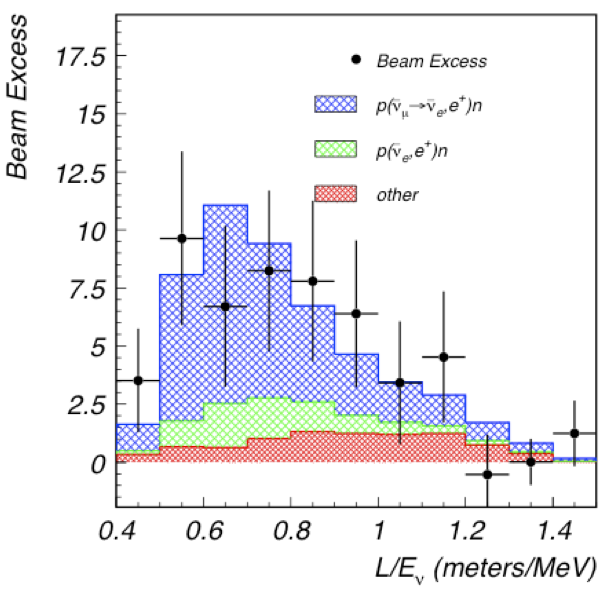
\includegraphics[width = \mediumfigwidth]{figures-chap2/LSND_excess.png}
    \caption[LSND excess.]{The \gls{lsnd} excess as a function of the neutrino L/E value. Events require a positron in the energy range $20 < E < 60$ MeV and a likelihood ratio of > 10 that the associated gamma was correlated (i.e. $\frac{\mathcal{L}_{\gamma}(correlated)}{\mathcal{L}_{\gamma}(accidental)} > 10$) \cite{LSND_excess}.}
    \label{fig:LSND excess}
\end{figure}
\newpage

\paragraph{MiniBooNE}
\gls{miniboone} collected data from the \gls{bnb} operating in both neutrino and antineutrino mode from 2002--2017. The \gls{bnb} is described in detail in \SectionRef{sec:BNB}. The detector was a sphere 12.2 m in diameter containing 818 tonnes of mineral oil. Charged particles in the oil would result in both Cherenkov and scintillation light that would be detected by 1520 \glspl{pmt} that surrounded the detector. The baseline from the \gls{bnb} source to \gls{miniboone} was 541 m.

Similar to \gls{lsnd}, \gls{miniboone} was searching for $\overset{(-)}{\nu}_{\!\!e}$ appearance from a predominantly $\overset{(-)}{\nu}_{\!\!\mu}$ beam. In neutrino mode, \gls{miniboone} observed an excess of 381.2\pm85.2 \gls{ccqe} events from an exposure of $12.84 \times 10^{20}$ \gls{pot} which corresponds to a 4.5$\sigma$ excess. This is shown in \FigureRef{fig:miniboone_sciboone}. Combining this with the antineutrino data from an exposure of $11.27 \times 10^{20}$ \gls{pot}, an excess of 460.5\pm99.0 \gls{ccqe} events (4.7$\sigma$) were observed. The excess of (anti)neutrinos considered were in the energy range of $200 < E_\nu < 1250$ MeV. The minimum energy of 200 MeV was chosen due to requiring a visible Cherenkov ring from a muon as a result of \numu \gls{ccqe} interactions which were used to constrain \nue events, whereas the maximum value of 1250 MeV was chosen to give a small value of L/E. Some of the most substantial backgrounds are due to $\overset{(-)}{\nu}_{\!\!e}$ events resulting from muon and kaon decays as well as \gls{nc} $\pi^0$ and \gls{nc} $\gamma$ events which mimic signal events. The intrinsic $\overset{(-)}{\nu}_{\!\!e}$'s are constrained by a joint fit of $\overset{(-)}{\nu}_{\!\!\mu}$ and $\overset{(-)}{\nu}_{\!\!e}$ assuming that $\overset{(-)}{\nu}_{\!\!\mu}$ disappearance is negligible, whilst the $\overset{(-)}{\nu}_{\!\!e}$'s from kaon decays are constrained by results from \gls{sciboone} and fits to kaon production data. Events from \gls{nc} interactions are constrained using \gls{miniboone} data. 

A two neutrino model was assumed so that a comparison with \gls{lsnd} data can be made, however, this results in the appearance and disappearance data not being compatible with one another. This may be resolved by assuming a different model to the 3+1 neutrino framework. The results are consistent with those seen by \gls{lsnd} and again point to the existence of additional neutrino flavours beyond the three predicted by the \gls{sm} \cite{MiniBooNE_excess}. 


The combined sensitivity results for a \numu disappearance search at the 90\% confidence limit from the \gls{miniboone} and \gls{sciboone} collaborations and a \gls{miniboone} only analysis (along with other experimental results) are shown on the right of \FigureRef{fig:miniboone_sciboone} \cite{MiniBooNE/SciBooNE_numu_disapp_contour}.
\begin{figure}
    \centering
    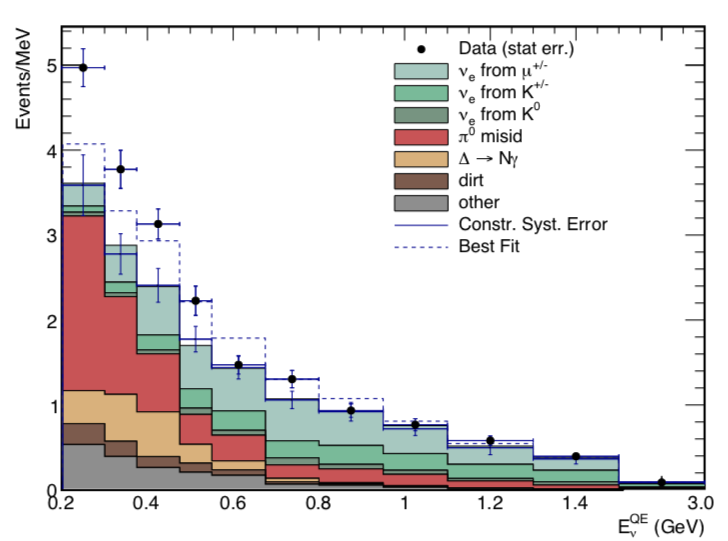
\includegraphics[width = \smallfigwidth, height = 0.9\smallfigwidth]{figures-chap2/MiniBooNE_excess.png}
    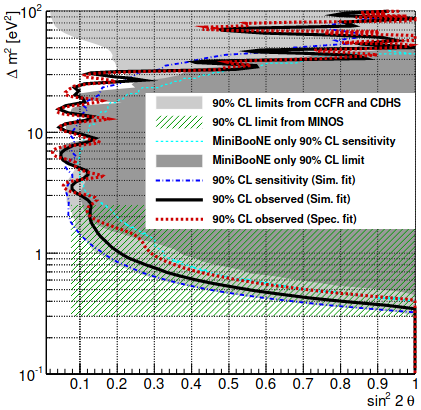
\includegraphics[width = \smallfigwidth, height = 0.9\smallfigwidth]{figures-chap2/numu_disapp_MiniBooNE_SciBooNE.png}
    \caption[\gls{miniboone}  excess and the \numu disappearance sensitivites from a simultaneous fit of \gls{miniboone}  and \gls{sciboone}  data.]{Left: The \gls{miniboone} excess from \nue \gls{ccqe} events. The best fit line assumed two neutrino oscillations \cite{MiniBooNE_excess}. Right: \numu disappearance exclusion contours obtained from the simultaneous fit of MiniBooNE and SciBooNE data along with other experimental results \cite{MiniBooNE/SciBooNE_numu_disapp_contour}.}
    \label{fig:miniboone_sciboone}
\end{figure}

\newpage
\paragraph{Gallium Anomaly}
The \textit{Gallium Anomaly} refers to the apparent deficit of electron neutrinos observed by placing radioactive sources which decay via electron capture in the solar neutrino experiments, \gls{sage} and \gls{gallex}. The \gls{gallex} experiment utilised two separate $^{51}$Cr neutrino sources. The key measured quantity was the production of $^{71}$Ge due to the transformation of $^{71}$Ga via inverse beta decay. The strength of the $^{51}$Cr neutrino sources was measured directly and via the production of $^{71}$Ge. The combined ratio of the strength of the two sources was found to be 0.93\pm0.08 \cite{GALLEX}. A later reanalysis of the results from \gls{gallex} with new technical data gave a ratio of 0.902\pm0.078 \cite{Gallex_reanalysis}. Similar to the \gls{gallex} experiment, the \gls{sage} experiment also compared the strength of a neutrino source from direct measurements and the production of $^{71}$Ge. \gls{sage} used both a $^{51}$Cr and a $^{37}$Ar source.  \gls{sage} observed a ratio 0.95\pm0.12 for the $^{51}$Cr source and a ratio of $0.79^{+0.09}_{-0.10}$ for the $^{37}$Ar source. The weighted average from the results from the two sources from \gls{sage} and the reevaluated values from the two \gls{gallex} sources is 0.88\pm0.05 \cite{SAGE}. This is consistent with a 2.3$\sigma$ significance and is consistent with \nuebar disappearance due to mixing with a sterile neutrino \cite{gallium_anomaly}.

\paragraph{Reactor Anomaly}
The \textit{Reactor Anomaly} refers to the apparent deficit of electron antineutrinos produced from neutron-rich fission products such as $^{235}$U, $^{238}$U, $^{239}$Pu and $^{241}$Pu undergoing  $\beta$-decay. For most cases, this involves placing a detector within a 100m of a reactor and measuring the ratio of observed to predicted event rates. The predicted event rates rely on antineutrinos produced from many isotopes with some of decay pathways not being well understood, thus accurately modelling them becomes difficult. The two principle antineutrino flux modelling methods are the \textit{summation} method and the \textit{beta conversion} method \cite{Reactor_anomaly}\cite{snowmass_2021}.
 
The \textit{summation} method relies on $\beta$--decay information from nuclear databases. Antineutrino contributions from individual $\beta$--decay branches are first calculated followed by a weighted sum from all the fissioning isotopes. A clear source of uncertainty with this method is the reliance on nuclear databases which are sometimes incomplete or inaccurate \cite{snowmass_2021}. 

The \textit{beta conversion} method uses virtual decay branches that sum up to experimentally found beta spectrum for each fissioning isotope. The individual beta spectrum from each branch is converted to a antineutrino spectrum and then summed together to produce an antineutrino spectrum for each fissioning isotope. $\beta$--decay measurements have been performed for $^{235}$U, $^{239}$Pu and $^{241}$Pu \cite{snowmass_2021}.

Flux data from experiments in the 1980's to the 2000's was generally in agreement with the best predictions of the time. In 2011, new antineutrino flux predictions were performed using the \textit{summation} method for $^{238}$U and the \textit{beta conversion} method for $^{235}$U, $^{239}$Pu and $^{241}$Pu by Mueller \textit{et al.} and Huber. These new predictions were sufficiently different from previous estimations to lead to a $\sim5\%$ discrepancy between predictions and measurements which has been dubbed the reactor anomaly \cite{snowmass_2021}. 

The average ratio of observed to predicted events is 0.943\pm0.023. It is acknowledged that the reactor fluxes may not be perfectly understood which could be the cause for such a deficit, however, it should be noted that other experiments have observed similar deficits for comparable L/E ranges \cite{Reactor_anomaly}.

\paragraph{\gls{karmen}}
The \gls{karmen} experiment is associated with the ISIS neutron source which produced \numu's, \numubar's and \nue's with a mean baseline of 17.7 m from source to detector. The \numu's are produced mono-energetically at 30 MeV from decay at rest $\pi^+$'s whereas the \numubar's and \nue's have a continuous energy spectrum up to 52.8 MeV from decay at rest $\mu^+$. The lifetime of pions is much shorter than muons, meaning \numu's are easily distinguished from \numubar's and \nue's since there is a significant time difference between the detection of the two. The \gls{karmen} detector consists of 65 tons of liquid scintillator used to detect neutrinos. 7000 tons of steel along with a two layer veto counter provides shielding against cosmic and beam related backgrounds \cite{Upper_limits_for_neutrino_oscillations_numubar_to_nuebar_from_muon_decay_at_rest}. 

\gls{karmen} investigated both the $\numu \rightarrow \nue$  and  $\numubar \rightarrow \nuebar$ oscillation channels with the latter being the more sensitive channel due to no \nuebar's being produced by ISIS (other than by contamination) meaning that any \nuebar's detected would be from oscillations. The \nuebar's would be detected via inverse beta decay with protons in the scintillator with the signal being a prompt \positron followed by a delayed $\gamma$ as a result of neutron capture \cite{Upper_limits_for_neutrino_oscillations_numubar_to_nuebar_from_muon_decay_at_rest}. 

After applying the selection criteria, to the data collected between February 1997 to March 2001, 15 \nuebar candidate events were observed with the total background expectation being $(15.8\pm 0.5)$ events. Assuming that mixing is maximal and that $\Delta m^2 \geq 100$ eV$^2$ an oscillation signal of $(2913 \pm 269)$ events would be expected. The selection criteria include considering the timing information of the ISIS beam meaning the \positron must be detected within 0.6 and 10.6 $\mu$s of the beam window, the neutron capture must occur with a time delay between 5 and 300 $\mu$s, the \positron must deposit a minimum of 16 MeV of visible energy which removes neutral current contributions and the neutron capture event must have an energy below 8 MeV \cite{Upper_limits_for_neutrino_oscillations_numubar_to_nuebar_from_muon_decay_at_rest}.

\nue's are detected by \gls{cc} interactions with carbon-12 via
\begin{equation}
    \nue + {^{12}\text{C}} \longrightarrow {^{12}\text{N}} + \electron \\
    {^{12}\text{N}} \longrightarrow {^{12}\text{C}} + \positron + \nue,
\end{equation}
with the requirement that the \nue's are detected within the \numu beam time window. The signature for a \nue interaction is a prompt  monoenergetic \electron with 12.5 MeV kinetic energy (which is calculated from the inital energy of \numu and the mass difference between $^{12}$C and $^{12}$N) and a delayed \positron with energies up to 16.3 MeV (which is the $\beta$--decay end-point energy). In order to distinguish the \nue's from oscillations and those due to the decay of $\mu^+$, oscillated \nue's were only considered between 0--110 ns and 330--440 ns after the beam-on-target. Additionally, the \positron was required to have an energy between 3.5 and 16.5 MeV during a time window of 0.5--36.5 ms after the beam time. From the data collected between June 1990 and May 1994, 3 candidate events were found. With an oscillation signal, 158.4 events are to be expected \cite{Limits_on_neutrino_oscillations_in_the_appearance_channels_numu_to_nue_and_numubar_to_nuebar}. 

No evidence of oscillations was found from either channel, with the number of events observed being consistent with background predictions. 90\% confidence limit contours for both $\numu \rightarrow \nue$  and  $\numubar \rightarrow \nuebar$ are shown on the left of \FigureRef{fig:karmen_contours} from four years of data collected between 1990 and 1994. An updated $\numubar \rightarrow \nuebar$ 90\% confidence level exclusion contour is shown on the right of \FigureRef{fig:karmen_contours} from the data collected between 1997 and 2001 as well as external results from \gls{lsnd}, Bugey and CCFR \cite{LSND_excess}\cite{Upper_limits_for_neutrino_oscillations_numubar_to_nuebar_from_muon_decay_at_rest}\cite{Limits_on_neutrino_oscillations_in_the_appearance_channels_numu_to_nue_and_numubar_to_nuebar}\cite{Bugey}\cite{CCFR}.

\begin{figure}[h!]
    \centering
    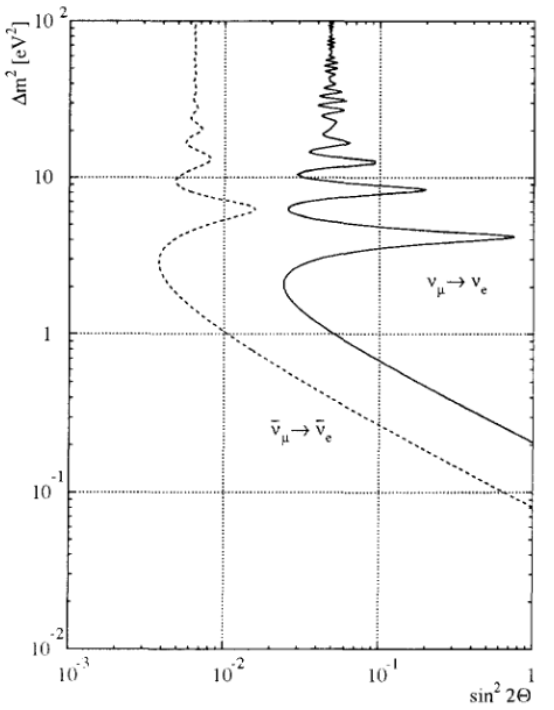
\includegraphics[width = \smallfigwidth, height = \smallfigwidth]{figures-chap2/karmen_contours.png}
    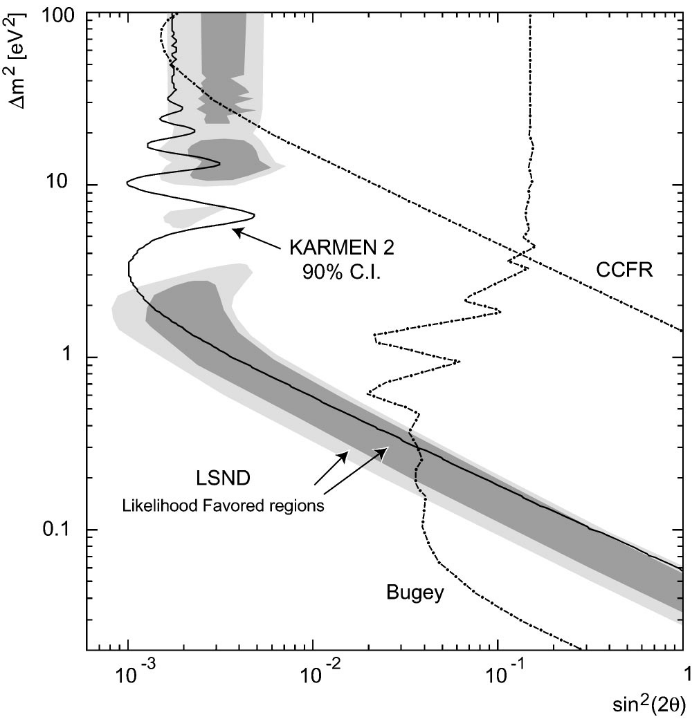
\includegraphics[width = \smallfigwidth, height = \smallfigwidth]{figures-chap2/karmen_contours_2.png}
    \caption[Exclusion contour from \gls{karmen} for \nue and \nuebar appearance.]{Left: Exclusion contours for $\numu \rightarrow \nue$  and  $\numubar \rightarrow \nuebar$ oscillations from data taken between 1990 and 1994 \cite{Limits_on_neutrino_oscillations_in_the_appearance_channels_numu_to_nue_and_numubar_to_nuebar}. Right: Updated Exclusion contours for $\numubar \rightarrow \nuebar$ oscillations from data taken between 1997 and 2001. External limits from \gls{lsnd}, Bugey and CCFR are also shown \cite{Upper_limits_for_neutrino_oscillations_numubar_to_nuebar_from_muon_decay_at_rest}.}
    \label{fig:karmen_contours}
\end{figure}

\paragraph{\gls{minos}}

The \gls{minos} experiment consisted of a near detector at a baseline of 1.04 km and a far detector at a baseline of 735 km and utilised the \gls{numi} beam. The \gls{numi} beam is muon-neutrino dominated and has a peak energy of 3 GeV. Therefore, \gls{minos} focused on measuring \numu \gls{cc} and \gls{nc} interactions from an exposure of $10.56 \times 10^{20}$ \gls{pot}. Both detectors consist of steel scintillator calorimeters that measure the charge and momentum of muons by the use of magnetic field. 

The \gls{nc} sample is selected by requiring that activity from interactions is contained on fewer than 47 steel scintillator planes as well as requiring the reconstructed track (if present) to not extend more than 5 planes beyond the hadronic shower. Additional criteria are applied to account for the reconstruction not being able to resolve coincident events. Only events that are rejected by the \gls{nc} selection are considered for the \gls{cc} selection. The \gls{cc} sample requires a contained interaction with a single outgoing muon track and the possible presence of hadronic shower. 

For the oscillation analysis, \gls{minos} assumed a (3+1) framework and used the full oscillation probabilities in vacuum (it was determined that including the matter effect had a negligible effect). Based on global data, $\sin^2{\theta_{12}}$ and $\Delta m^2_{41}$ were set to 0.307 and $7.54\times10^{-5}$ eV$^2$ respectively. $\sin^2{\theta_{13}}$ was set to 0.022 which was based on data from reactor experiments and $\theta_{13}$ was set to 0 since it had negligible impact on the analysis. The analysis also has negligible sensitivity to $\delta_{13,14,24}$, so all three were also set to 0. Parameters $\theta_{23}$, $\theta_{24}$, $\theta_{34}$, $\Delta m^2_{32}$ and $\Delta m^2_{41}$ are what are fit for in the analysis. 

Since \gls{minos} is sensitive to $10^{-3} \lesssim \Delta m^2 \lesssim 10^2$ eV$^2$, sterile oscillations may occur in both detectors. Due to this, the ratio of the energy spectrum in the far detector to the near detector are considered instead of using the near detector to predict the spectrum of the far detector. Both the \gls{cc} and \gls{nc} spectra are shown on the left of \FigureRef{fig:minos_spectra_contour} and show good agreement with a three neutrino model. Three flavour oscillations are consistent with the data at the 54.7\% confidence level with no indication of the presence of sterile neutrinos \cite{MINOS}. 

Following the results from \gls{minos}, it's successor, \gls{minos}+, was exposed to $5.80 \times 0^{20}$ \gls{pot} with a peak \numu energy of 7 GeV. \gls{minos}+ used the same detectors as \gls{minos}, but the analysis used a two detector fit instead of the ratio of energy spectra to obtain the sensitivity contours. The exclusion contours are produced in ($\sin^2{\theta_{24}}$, $\Delta m^2_{41}$) space where parameters $\theta_{23}$, $\theta_{34}$ and $\Delta m^2_{31}$ are varied to minimise the fit statistic with the results from the combined data from \gls{minos} and \gls{minos}+ being shown on the right of \FigureRef{fig:minos_spectra_contour} \cite{MINOS_numu_disapp_contour}.

\begin{figure}[h!]
    \centering
    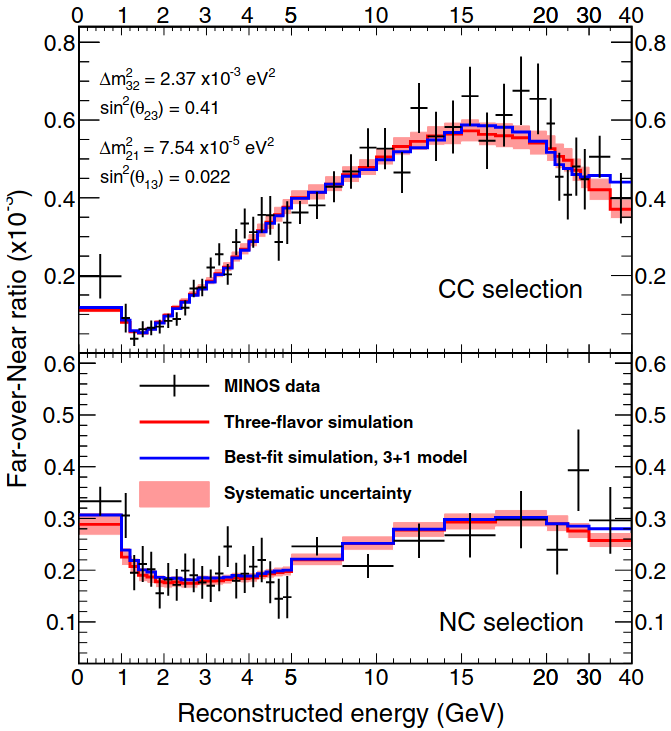
\includegraphics[width = \smallfigwidth, height = 1.1\smallfigwidth]{figures-chap2/minos_spectra.png}
    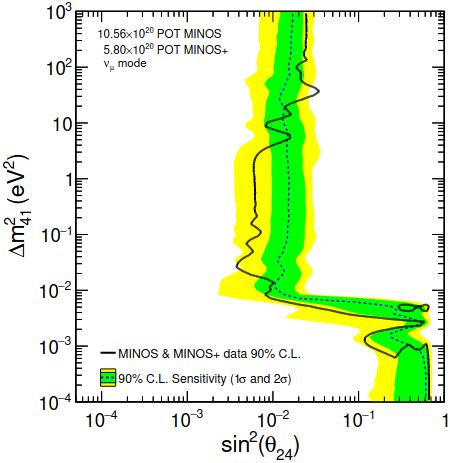
\includegraphics[width = \smallfigwidth, height = 1.1\smallfigwidth]{figures-chap2/numu_disapp_Minos.png}
    \caption[Ratio of energy spectra in the far and near detector of \gls{minos} plus exclusion contours ($\sin^2{\theta_{24}}$, $\Delta m^2_{41}$) space.]{Left: The ratio of energy spectra from the far detector to the near detector of \gls{minos} for both \gls{cc} and \gls{nc} samples \cite{MINOS}. Right: Exclusion contours from \gls{minos} at the 90\% and 95\% confidence level along with external limits \cite{MINOS_numu_disapp_contour}.}
    \label{fig:minos_spectra_contour}
\end{figure}

\paragraph{\gls{katrin}}

In addition to measuring the neutrino mass scale, the \gls{katrin} experiment has also produced exclusion contours for the possible existence of light sterile neutrinos from a (3+1) model. The experimental setup is essentially the same as that described in \SectionRef{sec:direct_mass_measurement}. The $\beta$-decay spectrum produced from tritium decay depends on the mass of the emitted electron neutrino which is a superposition of the relevant mass states. Due to the active mass states, $m_{1,2,3}$, having relatively similar masses their superposition can not be probed by \gls{katrin}, however, if a sterile neutrino with mass significantly greater than $m_{1,2,3}$ is present this would be observable. The total differential $\beta$-decay spectrum, $\dByd{\Gamma}{E}$, would be given by the superposition of the standard spectrum from just the three active neutrinos with $m_{\beta}$ being the corresponding effective electron neutrino mass and the spectrum from a sterile neutrino with mass $m_s$ as, 
\begin{equation}
    \frac{\diff\Gamma}{\diff E} = \cos^2{\theta} \frac{\diff\Gamma}{\diff E}(m_{\beta}^2) + \sin^2{\theta} \frac{\diff\Gamma}{\diff E}(m_s^2),
\end{equation}
where $\theta$ is the active-sterile mixing angle. The signature for the presence of a light sterile neutrino would be a \textit{kink} like feature in the $\beta$-decay spectrum as is shown in \FigureRef{fig:katrin_kink_beta_decay}. Due to the large mass of the $m_s$ it can be seen that the endpoint energy from the sterile neutrino is much less than that of the active neutrinos. Therefore, the spectrum would also be distorted at energies below the active neutrino endpoint energy minus $m_{s}$. \cite{A_novel_detector_system_for_KATRIN_to_search_for_keV_scale_sterile_neutrinos}.

\begin{figure}[h!]
    \centering
    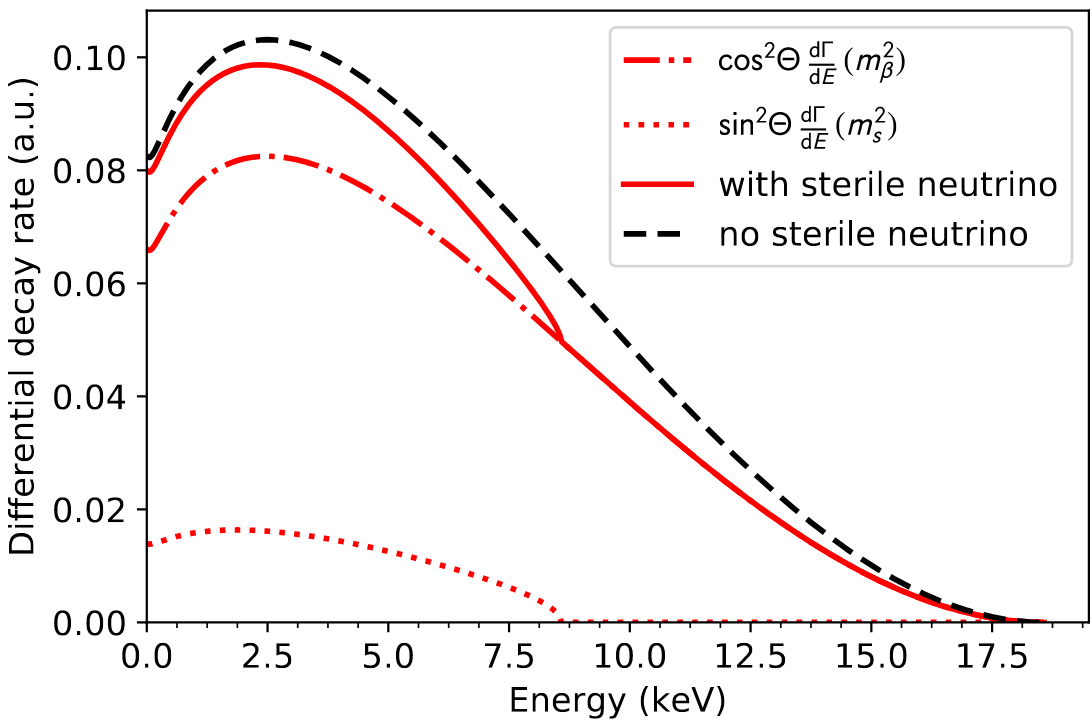
\includegraphics[width = \largefigwidth]{figures-chap2/KATRIN_kink.png}
    \caption[$\beta$-decay spectrum from tritium decay with the inclusion of the presence of a sterile neutrino.]{The $\beta$-decay spectrum from the decay of tritium showing the change in shape from due to the presence of 10 keV sterile neutrino and mixing angle of $\sin^2{\theta} = 0.2$ \cite{A_novel_detector_system_for_KATRIN_to_search_for_keV_scale_sterile_neutrinos}.}
    \label{fig:katrin_kink_beta_decay}
\end{figure}

From its second data collection period, \gls{katrin} has analysed $3.76 \times 10^6$ $\beta$-electrons from tritium decays and was sensitive to $m_4^2 \lesssim 1600$ eV$^2$ and $|U_{e4}|^2 \gtrsim 6 \times 10^{-3}$. No signal indicating the presence of light sterile neutrinos was observed and exclusion contours were produced at the 95\% confidence level. Two separate analyses were performed: one where the effective electron neutrino mass, $m_{\nu}^2$, was fixed to zero (which is justified since $m_4 \gg m_{1,2,3}$) and one where $m_{\nu}^2$ is an unconstrained nuisance parameter. The exclusion contours from both cases are shown in \FigureRef{fig:katrin_exclusion_contour} for data from the first and second campaign as well as both campaigns combined \cite{KATRIN_sterile_neutrino_results}. 

\begin{figure}[h!]
    \centering
    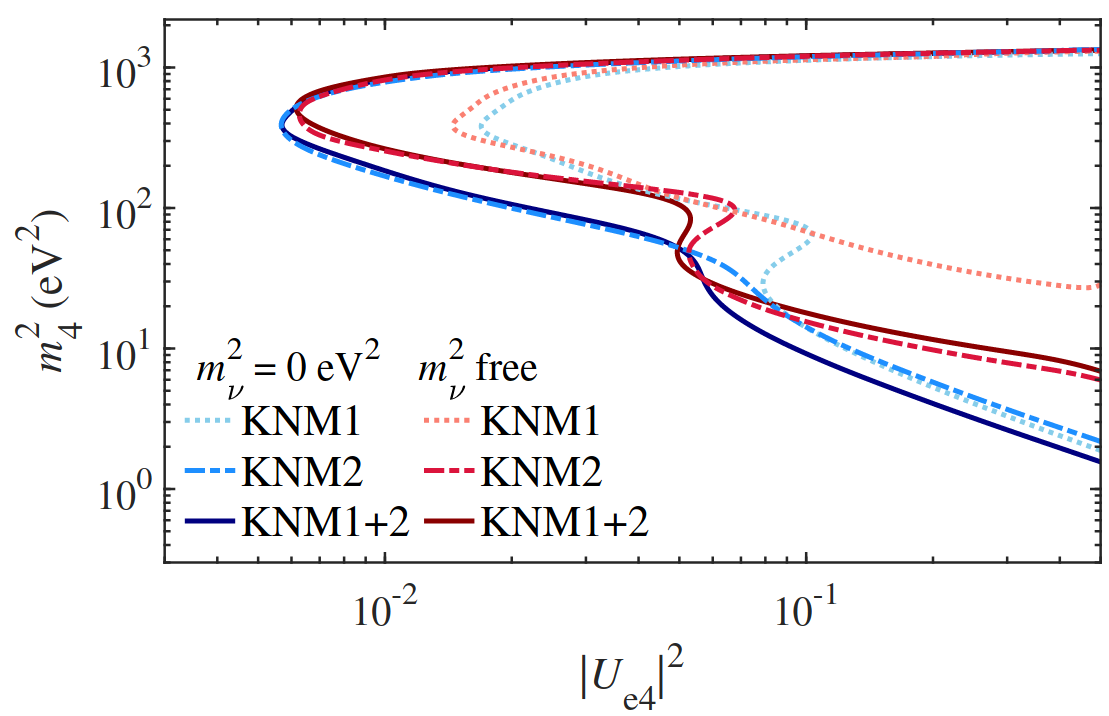
\includegraphics[width = \largefigwidth]{figures-chap2/KATRIN_exclusion_contours.png}
    \caption[\nue disappearance exclusion contours from the \gls{katrin} experiment.]{\nue disappearance exclusion contours from both data campaigns from the \gls{katrin} experiment as well as the combined data set. Both the case where the effective electron neutrino mass is fixed to 0 eV$^2$ and where it is a free parameter are considered \cite{KATRIN_sterile_neutrino_results}.}
    \label{fig:katrin_exclusion_contour}
\end{figure}


\paragraph{\gls{t2k}}
The near detector of the \gls{t2k} experiment, ND280, is located at 280 m from the neutrino beam source produced at J-PARC. Neutrino interactions occur with either a polystyrene scintillator or with water inside two fine grain detectors. Adjacent to the fine grain detectors are three \glspl{tpc} which are used to identify the particle type and momentum. Electromagnetic calorimeters which surround the detectors and \glspl{tpc} are used to distinguish showers and tracks \cite{T2K_nue_disapp_contour}. 

A \nue \gls{cc} event sample was selected by identifying electron candidates by use of both the \glspl{tpc} and the electromagnetic calorimeters. Backgrounds due to $\pi^0$ were reduced by rejecting events where a positive electron like track was observed within 10 cm of the electron and the \positron\electron invariant mass is less than 100 MeV/c$^2$. The selection efficiency of \nue \gls{cc} interactions was 26\% with a purity of 63\% \cite{T2K_nue_disapp_contour}. 

ND280 analysed data taken between January 2010 and May 2013 which corresponds to $5.9 \times 10^{20}$ \gls{pot} with the horn running in neutrino mode. A total of 614 \nue candidate events were observed with an expected number of $665 \pm 51_{(syst)}$ events assuming no oscillations. The reconstructed neutrino energy range considered is 0.2 - 10 GeV and and sensitivities are produced in $(sin^22\thetaee, \Delta m^2_{eff})$ parameters space using the Feldman-Cousins approach. The allowed regions at the 68\% and 90\% confidence level are shown alongside the exclusion region at the 95\% confidence level in \FigureRef{fig:nue_disapp_external}. The best fit point oscillation point is at $sin^2{2\thetaee} = 1$ and $\Delta m^2_{eff} = 2.05$ eV$^2$/c$^4$. The \textit{p}-value of the no oscillation hypothesis was determined to be 0.085 \cite{T2K_nue_disapp_contour}.

\begin{figure}[!h]
    \centering
    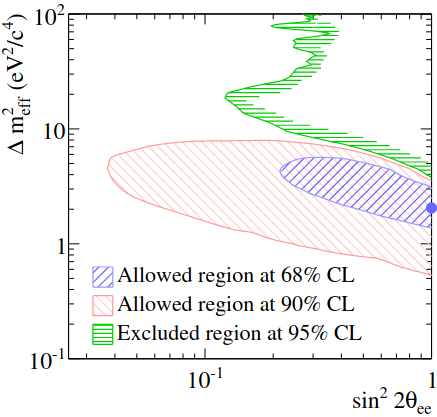
\includegraphics[width = \largefigwidth]{figures-chap2/nue_disapp_external_T2K.png}
    \caption[\nue disappearance limits from ND280.]{\nue disappearance exclusion and allowed regions from the near detector of the \gls{t2k} experiment, ND280 \cite{T2K_nue_disapp_contour}.}
    \label{fig:nue_disapp_external}
\end{figure}

\paragraph{IceCube}
Located close to the South Pole, the IceCube observatory is an ice-Cherenkov detector that is comprised of 5160 modules with each housing a number of \glspl{pmt}. The modules are located between 1450 and 2450 m below the ice surface. The majority of the detected neutrinos are produced from cosmic ray showers and have an energy ranging from 10 GeV to 1 PeV. To avoid backgrounds from high energy muons that may penetrate the ice sheet, the neutrino events selected are required to be upward going (i.e. originating from below the horizon) \cite{IceCube_numu_disapp_contour}.

A total of 305,735 \numu and \numubar events were analysed from 8 years of IceCube data under a (3+1) neutrino hypothesis. The results depend on both $\theta_{24}$ and $\theta_{34}$, but the contours have been produced under the assumption that $\theta_{34}$ and the \gls{cp} phases are set to zero. The results are shown in \FigureRef{fig:icecube} along with other experimental results. The left plot is the 90\% C.L. allowed region, whereas the right plot is the 99\% C.L. exclusion contour. The star in each plot represents the best-fit point. The best fit likelihood is found to be consistent with the no sterile neutrino oscillation with a \textit{p}-value of 8\% \cite{IceCube_numu_disapp_contour}.



\begin{figure}[h!]
    \centering
    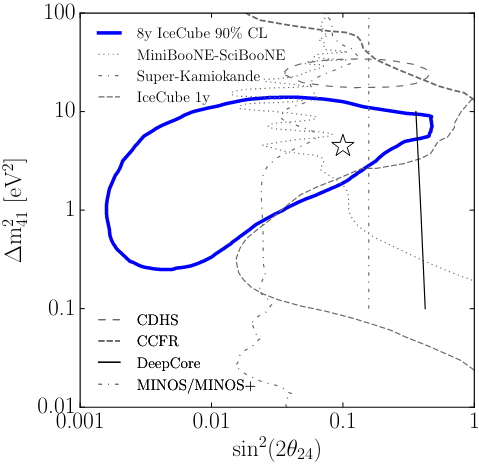
\includegraphics[width = 0.49\textwidth]{figures-chap6/external_limits/numu_disapp_icecube_90pct.png}
    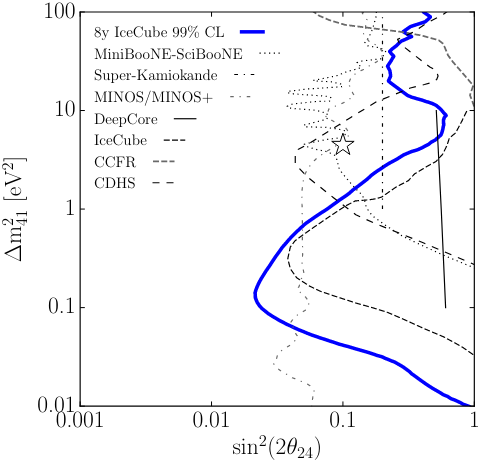
\includegraphics[width = 0.49\textwidth]{figures-chap6/external_limits/numu_disapp_icecube_99pct.png}
    \caption[\nue disappearance limits from the IceCube experiment.]{\numu disappearance results from the 8 years of IceCube data. The 90\% allowed region (Left) and the 99\% exclusion region (right) are shown under the assumption that $\theta_{34} = 0$ \cite{IceCube_numu_disapp_contour}.}
    \label{fig:icecube}
\end{figure}

\newpage
\paragraph{\gls{microboone}}
The \gls{microboone} experiment was designed to investigate the low energy excess of events observed by the \gls{miniboone} collaboration. A detailed description of the \gls{microboone} detector can be found in \SectionRef{sec:MicroBooNE}. \gls{microboone} analysed data from the \gls{bnb} running in neutrino mode between February 2016 and July 2018 which corresponds to an exposure $\sim 7 \times 10^{20}$ \gls{pot}. A single $\gamma$ analysis along with three separate single \electron from \nue interaction analyses were performed, each classified by the event topology and reconstruction method namely, 
\begin{itemize}
    \item $1\gamma0p, 1\gamma1p$ (0 lepton) final state from a $\Delta$ baryon decay with Pandora being used for reconstruction. 
    \item $1\electron1p(0\pi)$ two-body \gls{ccqe} scattering final state using a deep learning approach to perform the reconstruction.
    \item $1\electron Np0\pi, 1\electron0p0\pi$ (pionless) final state using Pandora to perform the reconstruction. 
    \item $1\electron X$ inclusive scattering final state using Wire-Cell to perform the reconstruction.
\end{itemize}

The production of single photon events (with no charged leptons or pions in the final state) at \gls{bnb} energies is dominated by the neutrino induced \gls{nc} $\Delta(1232) \rightarrow N\gamma$ decay, where \textit{N} represents either a proton or neutron. The analysis searches for a single photon shower with either a single visible proton or no other visible activity which are labelled $1\gamma1p$ and $1\gamma0p$ respectively. The Pandora reconstruction framework is used to classify events as either track or shower like events, followed by identifying topologies with one shower and either zero or one associated track which define the two 1$\gamma$ selections. The analysis requires that candidate events are fully contained in the fiducial volume as well as applying cuts on the shower energy, properties of the track and shower opening angle which ensures sufficient reconstruction performance as well as rejecting some backgrounds. A number of \glspl{bdt} are then used on the remaining events to further reduce backgrounds from cosmic muons, $\pi^0$ decays, \nue \gls{cc} events and \numu \gls{cc} events \cite{Search_for_Neutrino_Induced_Neutral_Current_Delta_Radiative_Decay_in_MicroBooNE_and_a_First_Test_of_the_MiniBooNE_Low_Energy_Excess_under_a_Single_Photon_Hypothesis}. 

The dominant background in this search is due to $\Delta \rightarrow N \pi^0$ where the pion decays into two photons. If one of the photons is not reconstructed the event may mimic a single photon event. Possible reasons a photon may not be reconstructed include: the pion decay being very asymmetric leading to one low energy $\gamma$ that is not reconstructed, the emission of the two photons is highly co-linear meaning the two photons are reconstructed as a single shower, one of the photons exits the \gls{tpc} before interacting or one of the photons may be poorly reconstructed (due to unresponsive wires). In order to constrain this background, a $2\gamma1p$ and $2\gamma0p$ sample are also selected \cite{Search_for_Neutrino_Induced_Neutral_Current_Delta_Radiative_Decay_in_MicroBooNE_and_a_First_Test_of_the_MiniBooNE_Low_Energy_Excess_under_a_Single_Photon_Hypothesis}. 

For the $1\gamma1p$ sample, 16 events were observed with a background prediction of $20.5 \pm 3.6_{(syst)}$, whereas for the $1\gamma0p$ sample, 153 events were observed with a background prediction of $145.1 \pm 13.8_{(syst)}$. This is shown in \FigureRef{fig:microboone_1gamma} where the $1\gamma1p$ and $1\gamma0p$ analyses are shown in the left and right plots respectively. This analysis disfavours the single photon interpretation of the \gls{miniboone} low energy excess and instead favours the nominal prediction at the 94.8\% confidence level \cite{Search_for_Neutrino_Induced_Neutral_Current_Delta_Radiative_Decay_in_MicroBooNE_and_a_First_Test_of_the_MiniBooNE_Low_Energy_Excess_under_a_Single_Photon_Hypothesis}. 

\begin{figure}[h!]
    \centering
    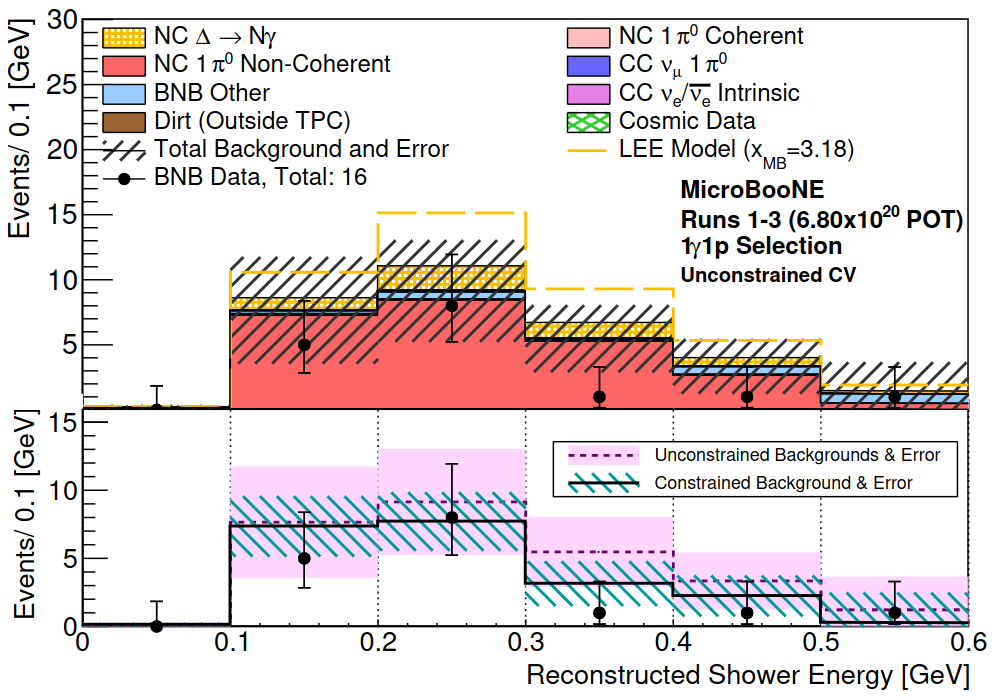
\includegraphics[width = \smallfigwidth]{figures-chap2/microboone_1gamma_1p.png}
    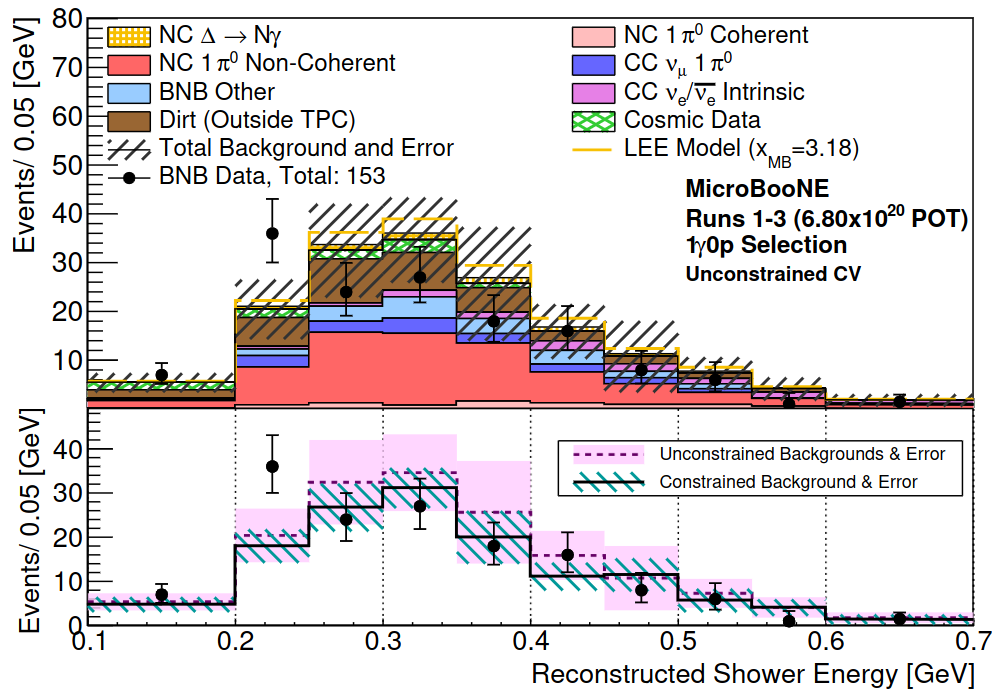
\includegraphics[width = \smallfigwidth]{figures-chap2/microboone_1gamma0p.png}
    \caption[Reconstructed shower energy spectra for the \gls{microboone} $1\gamma1p$ (left) and $1\gamma0p$ (right) analyses.]{The reconstructed shower energy spectra for the \gls{microboone} $1\gamma1p$ (left) and $1\gamma0p$ (right) analyses. In each case the top section shows the breakdown of the unconstrained background prediction whereas the bottom section shows the total unconstrained background as well as the background after the $2\gamma$ constraint has been applied \cite{Search_for_Neutrino_Induced_Neutral_Current_Delta_Radiative_Decay_in_MicroBooNE_and_a_First_Test_of_the_MiniBooNE_Low_Energy_Excess_under_a_Single_Photon_Hypothesis}.}
    \label{fig:microboone_1gamma}
\end{figure}


The $1\electron1p$ \gls{ccqe} topology is expected to dominate at energies below 500 MeV. The analysis only considers fully contained \nue or \numu interactions with a lepton and proton in the final state. \glspl{cnn} are used to distinguish track and shower like images as well as determining particle species. A \gls{bdt} uses kinematic and topological variables to produce a \gls{ccqe} event sample followed by a CNN to select the final candidates. The reconstructed neutrino energy range considered is 200--1200 MeV. 25 \nue candidate events were selected in this energy range which is in agreement with the background prediction of $29.0 \pm 1.9_{(sys)} \pm 5.4_{(stat)}$ events which is shown in \FigureRef{fig:microboone_machine_learning}. By mapping the low energy excess observed by \gls{miniboone} to \gls{microboone}, 11.6 \nue events are expected in addition to the background prediction which is not observed in this analysis \cite{Search_for_an_Excess_of_Electron_Neutrino_Interactions_in_MicroBooNE_Using_Multiple_Final_State_Topologies}\cite{Search_for_an_anomalous_excess_of_charged_current_quasi_elastic_nue_interactions_with_the_MicroBooNE_experiment_using_Deep_Learning_based_reconstruction}. 

\begin{figure}[h!]
    \centering
    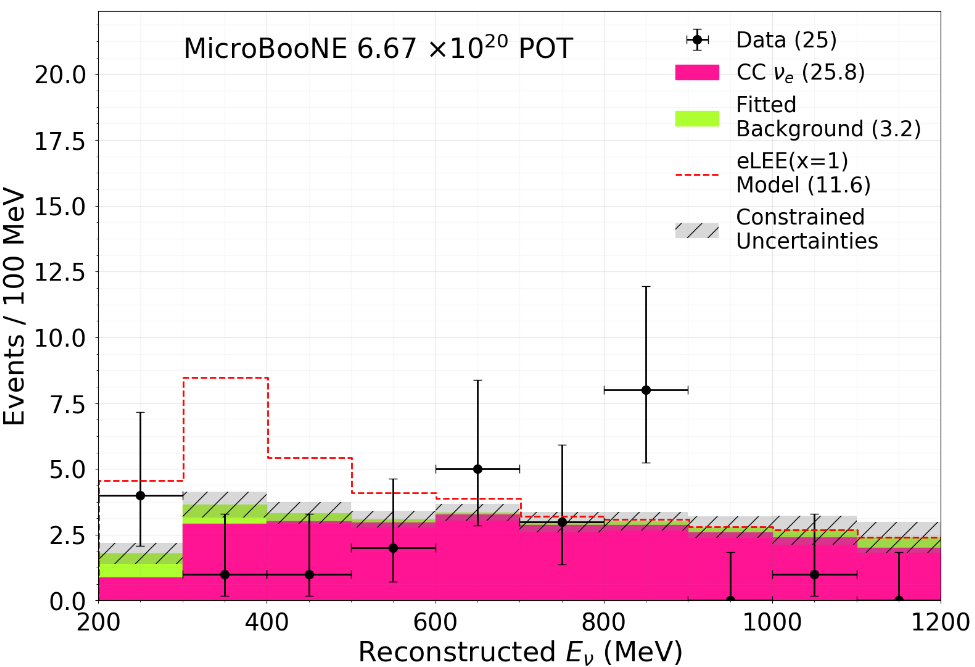
\includegraphics[width = \largefigwidth]{figures-chap2/microboone_machine_learning.png}
    \caption[Reconstructed neutrino energy from \gls{microboone} data using a \gls{ccqe} $1\electron1p(0\pi)$ final state topology for a \nue analysis.]{The reconstructed neutrino energy from a $1\electron1p(0\pi)$ \gls{ccqe} final state topology using a deep learning approach to analyse \gls{microboone} data. Background events include cosmic and \numu interactions
    \cite{Search_for_an_Excess_of_Electron_Neutrino_Interactions_in_MicroBooNE_Using_Multiple_Final_State_Topologies}.}
    \label{fig:microboone_machine_learning}
\end{figure}

The pionless final state analysis considers two sub-topologies: one with a single electron plus one or more visible protons and one with a single electron and no visible protons. Pandora is used in conjunction with other tools to reconstruct events and remove cosmic ray background events. Combining these two topologies is the exact signal event signature that \gls{miniboone} used. The reconstructed neutrino energy range considered is 10--2390 MeV. 64 \nue events were observed from the $1\electron Np0\pi$ channel which had a background prediction of $86.8 \pm 8.8_{(stat)} \pm 11.5_{(syst)}$ events. The $1\electron 0p0\pi$ channel instead observed 34 \nue events with a background prediction of $30.2 \pm 5.6_{(stat)} \pm 4.3_{(syst)}$ events which are shown in \FigureRef{fig:microboone_pionless}. The $1\electron Np0\pi$ result rejects the \gls{miniboone} low energy excess at a 97.9\% confidence level. The $1\electron 0p0\pi$ channel has an excess of events in the lowest energy region and does not fully exclude the hypothesis that \nue \gls{cc} interactions caused the low energy excess, however, it is the least sensitive channel to the \gls{miniboone} excess \cite{Search_for_an_Excess_of_Electron_Neutrino_Interactions_in_MicroBooNE_Using_Multiple_Final_State_Topologies} \cite{Search_for_an_anomalous_excess_of_charged_current_nue_interactions_without_pions_in_the_final_state_with_the_MicroBooNE_experiment}. 

\begin{figure}[h!]
    \centering
    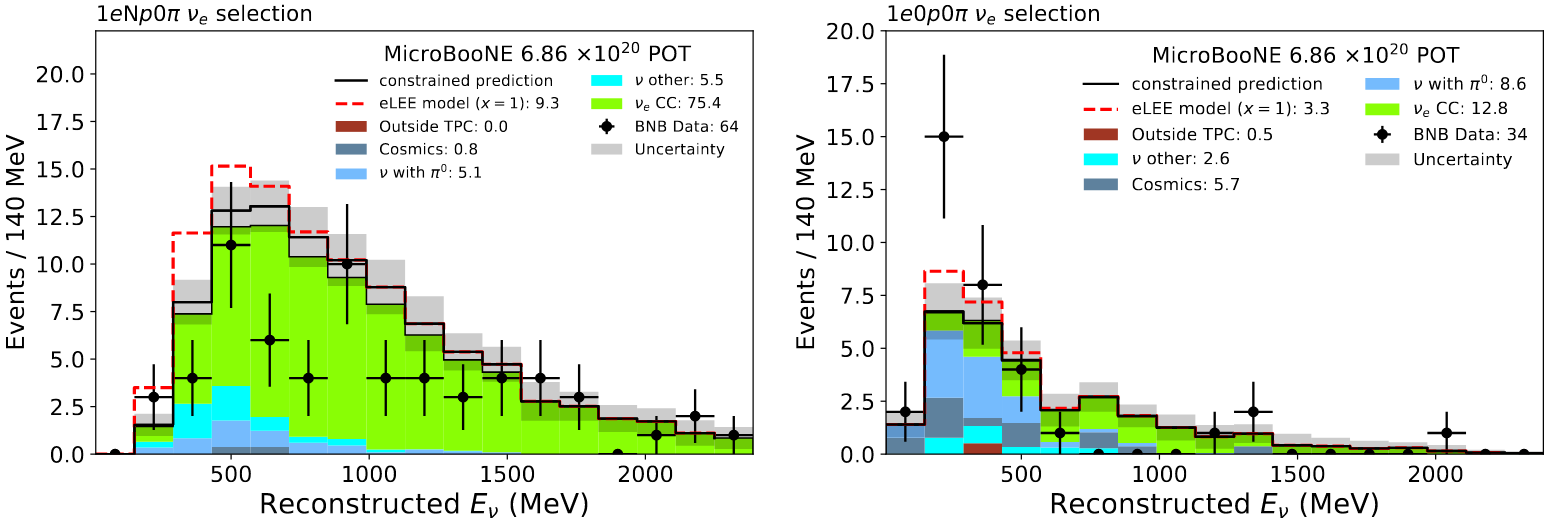
\includegraphics[width =\hugefigwidth]{figures-chap2/microboone_pionless.png}
    \caption[Reconstructed neutrino energy from \gls{microboone} data using pionless final state topology for a \nue analysis.]{The reconstructed neutrino energy from a pionless final state topology (Left: $1\electron Np0\pi$, Right $1\electron 0p0\pi$) using Pandora for event reconstruction to analyse \gls{microboone} data \cite{Search_for_an_Excess_of_Electron_Neutrino_Interactions_in_MicroBooNE_Using_Multiple_Final_State_Topologies}.}
    \label{fig:microboone_pionless}
\end{figure}

The inclusive topology considers all hadronic final states and therefore has the largest statistics. Wire-Cell, which creates 3D images from 1D wire position tomography is used for the reconstruction. Clustering algorithms and rejection tools are used on the images along with a deep neural network to identify the neutrino vertex and characterise the event. The analysis considers events in the 0 -- 2500 MeV neutrino energy range. Constraints coming from selected \numu \gls{cc} events and both \gls{cc} and \gls{nc} events with a reconstructed $\pi^0$ are used to improve the sensitivity and reduce systematic uncertainties. Following the \nue analysis and applying these constraints, 338 candidate \nue \gls{cc} events were observed which is a slight deficit with the predicted number of $(384.9 \pm 19.2_{(stat)} \pm 15.9_{(syst)})$ nominal events which is shown in \FigureRef{fig:microboone_inclusive}. An additional 37 events are predicted by applying the low energy excess observed by \gls{miniboone}.

\begin{figure}[h!]
    \centering
    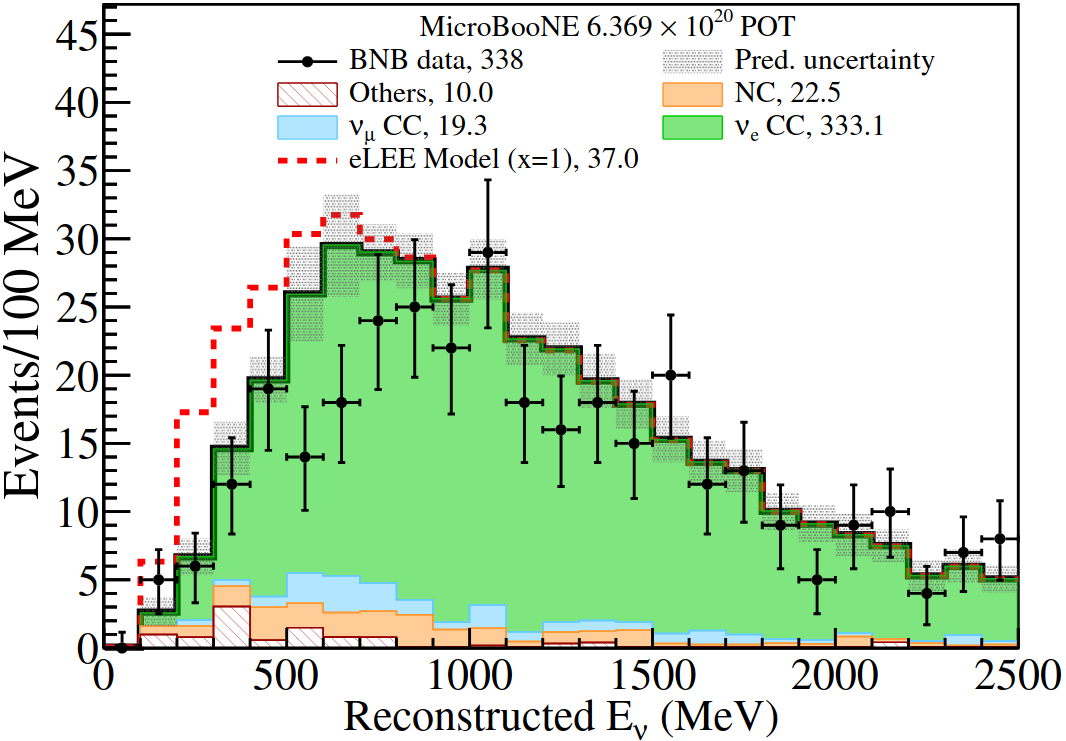
\includegraphics[width = \largefigwidth]{figures-chap2/microboone_inclusive.png}
    \caption[Reconstructed neutrino energy from \gls{microboone} data using an inclusive final state topology for a \nue analysis.]{The reconstructed neutrino energy from an inclusive final state topology using Wire-Cell for event reconstruction to analyse \gls{microboone} data\cite{Search_for_an_Excess_of_Electron_Neutrino_Interactions_in_MicroBooNE_Using_Multiple_Final_State_Topologies}.}
    \label{fig:microboone_inclusive}
\end{figure}


Interpreting the most recent \gls{microboone} results in terms of the allowed regions preferred by \gls{miniboone}, it is found that \gls{microboone} excludes a significant portion of the parameter space, but not the entire region. Both the inclusive and \gls{ccqe} channels from \gls{microboone} are shown alongside the \gls{miniboone} results at the $3\sigma$ confidence level in \FigureRef{fig:microboone_exclusion_contour}. The detection efficiency of \gls{ccqe} events decreases at higher energies for both \gls{microboone} and \gls{miniboone} which is not the case for the inclusive channel, hence the latter provides a significantly stronger constraint. While the above analyses have only considered about half of the \gls{microboone} data, it is not expected that using the full data set will significantly change the results. This is due to the number of observed events in the inclusive data showing a deficit when compared to the background events leading to a stronger constraint \cite{MicroBooNE_and_the_nue_Interpretation_of_the_MiniBooNE_Low_Energy_Excess}.
\begin{figure}[h!]
    \centering
    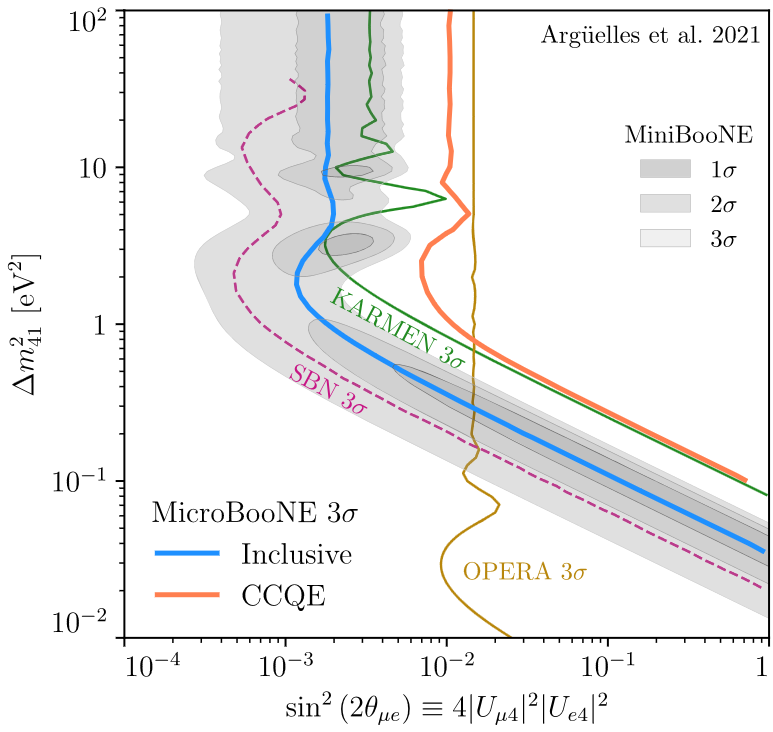
\includegraphics[width = \largefigwidth]{figures-chap2/microboone_exclusion_contour.png}
    \caption[\nue appearance exclusion contours from \gls{microboone} compared with the results from \gls{miniboone}.]{\nue appearance exclusion contours from \gls{microboone} data for both inclusive and \gls{ccqe} channels at the $3\sigma$ confidence level. The allowed regions from \gls{miniboone} are shown for comparison. \gls{microboone} excludes much of the region favoured by \gls{miniboone} but not the entire parameter space \cite{MicroBooNE_and_the_nue_Interpretation_of_the_MiniBooNE_Low_Energy_Excess}.}
    \label{fig:microboone_exclusion_contour}
\end{figure}

\newpage
\paragraph{\gls{stereo}}
The \gls{stereo} experiment is situated a few metres from the Institut Laue–Langevin research reactor in Grenoble. The detector consists of 6 cells filled with 1.8 m$^3$ of gadolinium doped liquid scintillator which acts as the target and measures the antineutrino energy spectrum as a result of the fission of uranium-235. \glspl{pmt} located at the top of each cell are used to detect the scintillation light. A water Cherenkov detector surrounds the cells which is used to identify cosmic muons which are passing through the detector. The 6 cells are positioned in a line along the axis of the reactor meaning each cell is at a slightly different baseline from the reactor (the baseline ranges from around 9 to 11 metres). 

The antineutrinos produced by the reactor are detected via inverse beta decay with the signature being a prompt signal from the positron a delayed signal when the neutron is captured by the gadolinium followed by photon cascade due to the de-excitation of the gadolinium. After selection cuts, \gls{stereo} detected and average of 394 antineutrinos per day and a total of 107,588 antineutrinos from two data taking periods over 3 years.  

The independent spectra from each of the 6 cells was compared with a given hypothesis where all parameters other than $\sin^22\theta_{ee}$ and $\Delta m^2_{41}$ were allowed to float in the fit. Exclusion contours at the 95\% confidence level produced from \gls{stereo} data following a Feldman Cousins' and Gaussian confidence level approach are shown in \FigureRef{fig:stereo_exclusion_contour}. Additionally, the allowed region and best fit point from reactor antineutrino anomaly data is shown. \gls{stereo} data is compatible with a no oscillation hypothesis, excludes much of the reactor antineutrino anomaly allowed region up to $\Delta m^2_{41} = \sim 5$ eV$^2$ as well as excluding the best fit points from Neutrino-4 and the NEOS-RENO collaborations at a $\sim 3\sigma$ level \cite{STEREO}. 

\begin{figure}[h!]
    \centering
    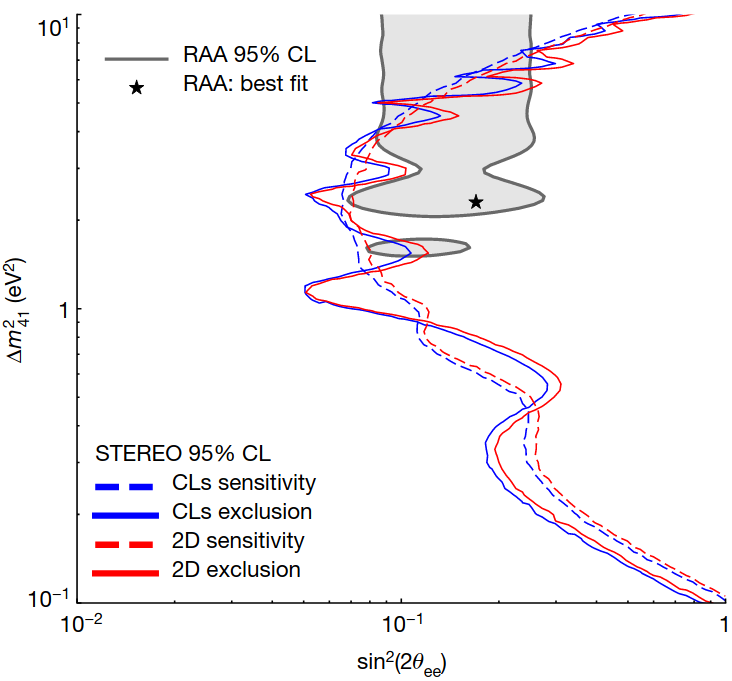
\includegraphics[width = \mediumfigwidth]{figures-chap2/stereo.png}
    \caption[\gls{stereo} exclusion sensitivity at the 95\% confidence level.]{The exclusion contour and exclusion sensitivity at the 95\% confidence level using both the Feldman-Cousins approach and the Gaussian Confidence Level method. The reactor antineutrino anomaly allowed region and best fit point are also shown \cite{STEREO}.}
    \label{fig:stereo_exclusion_contour}
\end{figure}


\newpage
\paragraph{Global Analysis}
A global analysis may be performed to encompass experimental data from a number of experiments into a single result. The \gls{lsnd} and \gls{miniboone} experiments push the results away from the \gls{sm} and towards a (3+1) model, however, the mixing angles required to explain the \gls{lsnd} and \gls{miniboone} excess are in tension with \numu disappearance data. The different allowed regions from a (3+1) model as well the combined region are shown on the left of \FigureRef{fig:allowed_exclusion_region_tension} with large portions of the allowed regions not being excluded by appearance data. The combined allowed region along with the exclusion region from disappearance experiments are shown on the right of \FigureRef{fig:allowed_exclusion_region_tension} with the entire allowed region being excluded by the disappearance contour. The level of tension between the allowed region and disappearance data has been quantified in terms of a \textit{p}-value of $3.7 \times 10^{-7}$, which strongly disfavours the (3+1) model. A caveat in the calculation of the \textit{p}-value is that the global fits have assumed that Wilks' theorem applies, however, it is not entirely clear if this is true for neutrino experiments \cite{snowmass_2021}\cite{wilks_theorem}. 

\begin{figure}
    \centering
    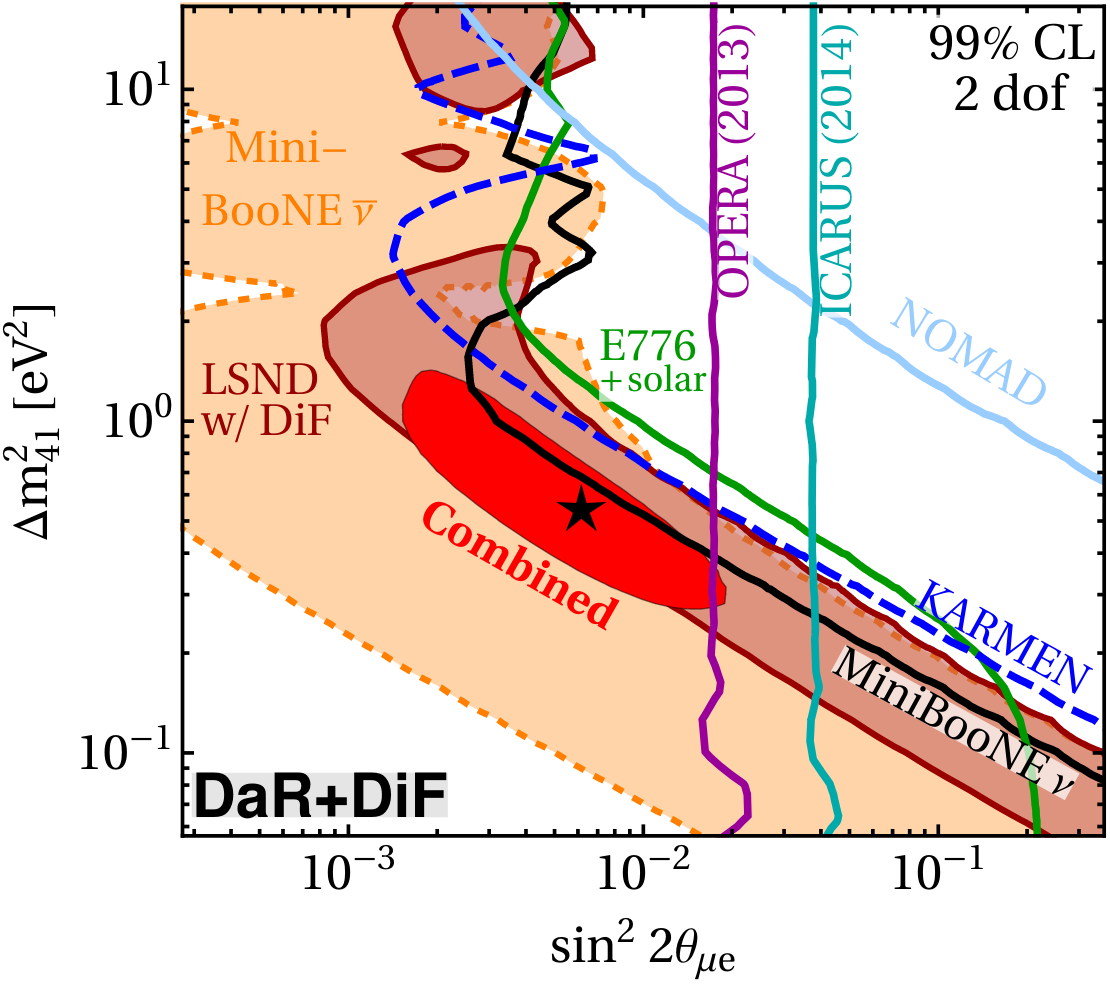
\includegraphics[width = \smallfigwidth, height = 0.885\smallfigwidth]{figures-chap2/nue_app_combo.png}
    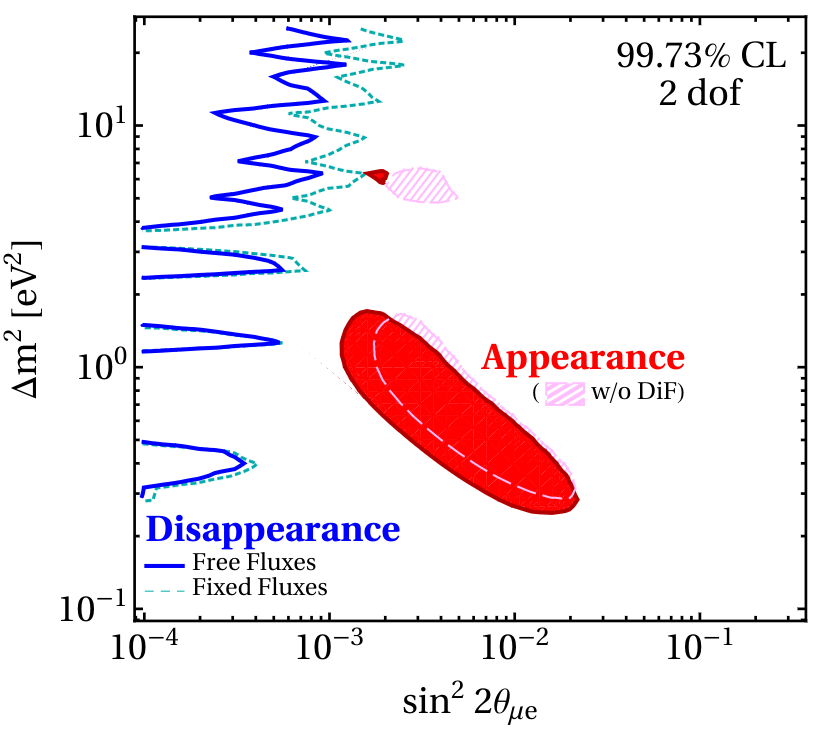
\includegraphics[width = \smallfigwidth, height = 0.9\smallfigwidth]{figures-chap2/preffered_exclusion_regions.png}
    \caption[Global analysis showing the allowed region from appearance experiments and the excluded region from disappearance experiments.]{Left: The allowed regions from \gls{lsnd} and \gls{miniboone} appearance signals as well as the combined region all at the 90\% confidence limit. Right: The preferred allowed region from appearance experiments as well as the excluded region from disappearance experiments at the 99.73\% confidence limit  \cite{LSND_KARMEN_nue_app_contour}.}
    \label{fig:allowed_exclusion_region_tension}
\end{figure}
